% !TEX root = main.tex

% TODO:
% REMARK:
% . * Don't mention LHC, CMS, etc. in this section, just have a historical review ana provide physical motivation to the study

\section{Events Selection and Reconstruction}
\label{sec:EventSelReco}

	To calculate the asymmetry from top quark in $t\bar{t}$, there must be some selections to extract the $t\bar{t}$ sample from other background samples. Also, there would be several analysis strategies to recognize physical objects and pick them out. The chapter will do these discussion and make some comparison and organization.
	
	\subsection{Events Selection : Signal Region}
	\label{ssec:EvtSel_SR}

		In this analysis, doing reasearch by the channel of lepton + jets, which means 2 tops have different decay modes. One decays leptonically, and another decays hadronically. It is expected that the hadronically decay top can be constructed with 1 b-tagged jet and 2 non b-tagged jets and the other top can be constructed imcompletely with 1 b-tagged jet, 1 lepton with missing neutrino 4-momentum by detector issue. For the $\textbf{Signal Region(SR)}$, the region with selection cut to extract signal in an analysis, there are the selection cuts below:

		\begin{itemize}
  		\item 1 selected lepton which are a tight muon or a tight electron
  		\item 0 lepton pass veto criteria which are loose muon and loose electron criterion
  		\item $\geq$ 4 selected jets with passing medium jet criteria
  		\item exact 2 btagged jets in these selected jets
  		\item each selected jets are isolated from the selected lepton with $\Delta R$ > 0.4
		\end{itemize}

		The $\Delta R$ criteria here means the angle distribution between selected jets and selected lepton in $\phi - \eta$ phase space with $\Delta R$ > 0.4. This would avoid the confusing cases that the lepton is really coming from jets or that the jets have some correlation with lepton in reconstruction process... etc.

		\begin{equation}
		\Delta R = \sqrt{ (\eta_{jet} - \eta_{lep})^2 - (\phi_{jet} - \phi_{lep})^2 } > 0.4
		\end{equation}

		%%% also put on the diagrams of N_Jets N_BJets N_TightLep before selection to valify the selection cut!

		%%% --- TODO --- %%%
		% to do the lumi-weight things (?)

	\subsection{Events Reconstruction}
	\label{ssec:EvtReco}

		To reconstruct the semi-leptonic $t\bar{t}$ system, it is suggested that to reconstruct the top quark which decays hadronically. It's an advantage that we can avoid dealing with missing 4-momentum from neutrino decays from leptonic top. And under the SR selection, if we can reconstruct the top which decays hadronically, the decay objects of leptonic decay top would be picked up simultaneously. This is a direct and common way to correctly identify selected candidates.

		\subsubsection{$\chi^2_{min}$ Method}
		\label{sssec:minchi2_intro} 

			There are multiple combinations of 1 b-tagged jet and 2 non b-tagged jet in an event. And how do we reconstruct hadronically decay top? In known and published analysis, based on the reco-level invariant mass of top quark itself and the intermediate particle in decay - W boson, they are used as constraints to invariant mass which is reconstructed from each combination. With the defined $\chi^2_{min}$ value, which shows below:

			\begin{equation}
			\chi^2 = (\frac{m_{jjb}-m_{t}}{\sigma_{t}})^2 + (\frac{m_{jj}-m_{W}}{\sigma_{W}})^2
			\label{eq:chi2}
			\end{equation}
			where $m_{t}$, $m_{W}$, $\sigma_{t}$ and $\sigma_{W}$ are the mean and width of top quark and W boson, coming from artificial fitting with jets corresponding to real decay quark with generator information in simulation sample(in appendix****), which are 168.15GeV, 81.25GeV, 20.6GeV and 12.1GeV seperately. Back to the part of $\chi^2$, for each combination, $m_{jjb}$ is the invariant mass of 1 b-tagged jet and 2 non-btagged jets; $m_{jj}$ is the invariat mass of 2 non b-tagged jets which are same 2 jets in $m_{jjb}$. the combination who have the minimum ${\chi}^{2}$ value in all of them is chosen as physical obsects coming from hadronically decay top.


\begin{figure}[H]
\centering
	\subfigure[muon channel]{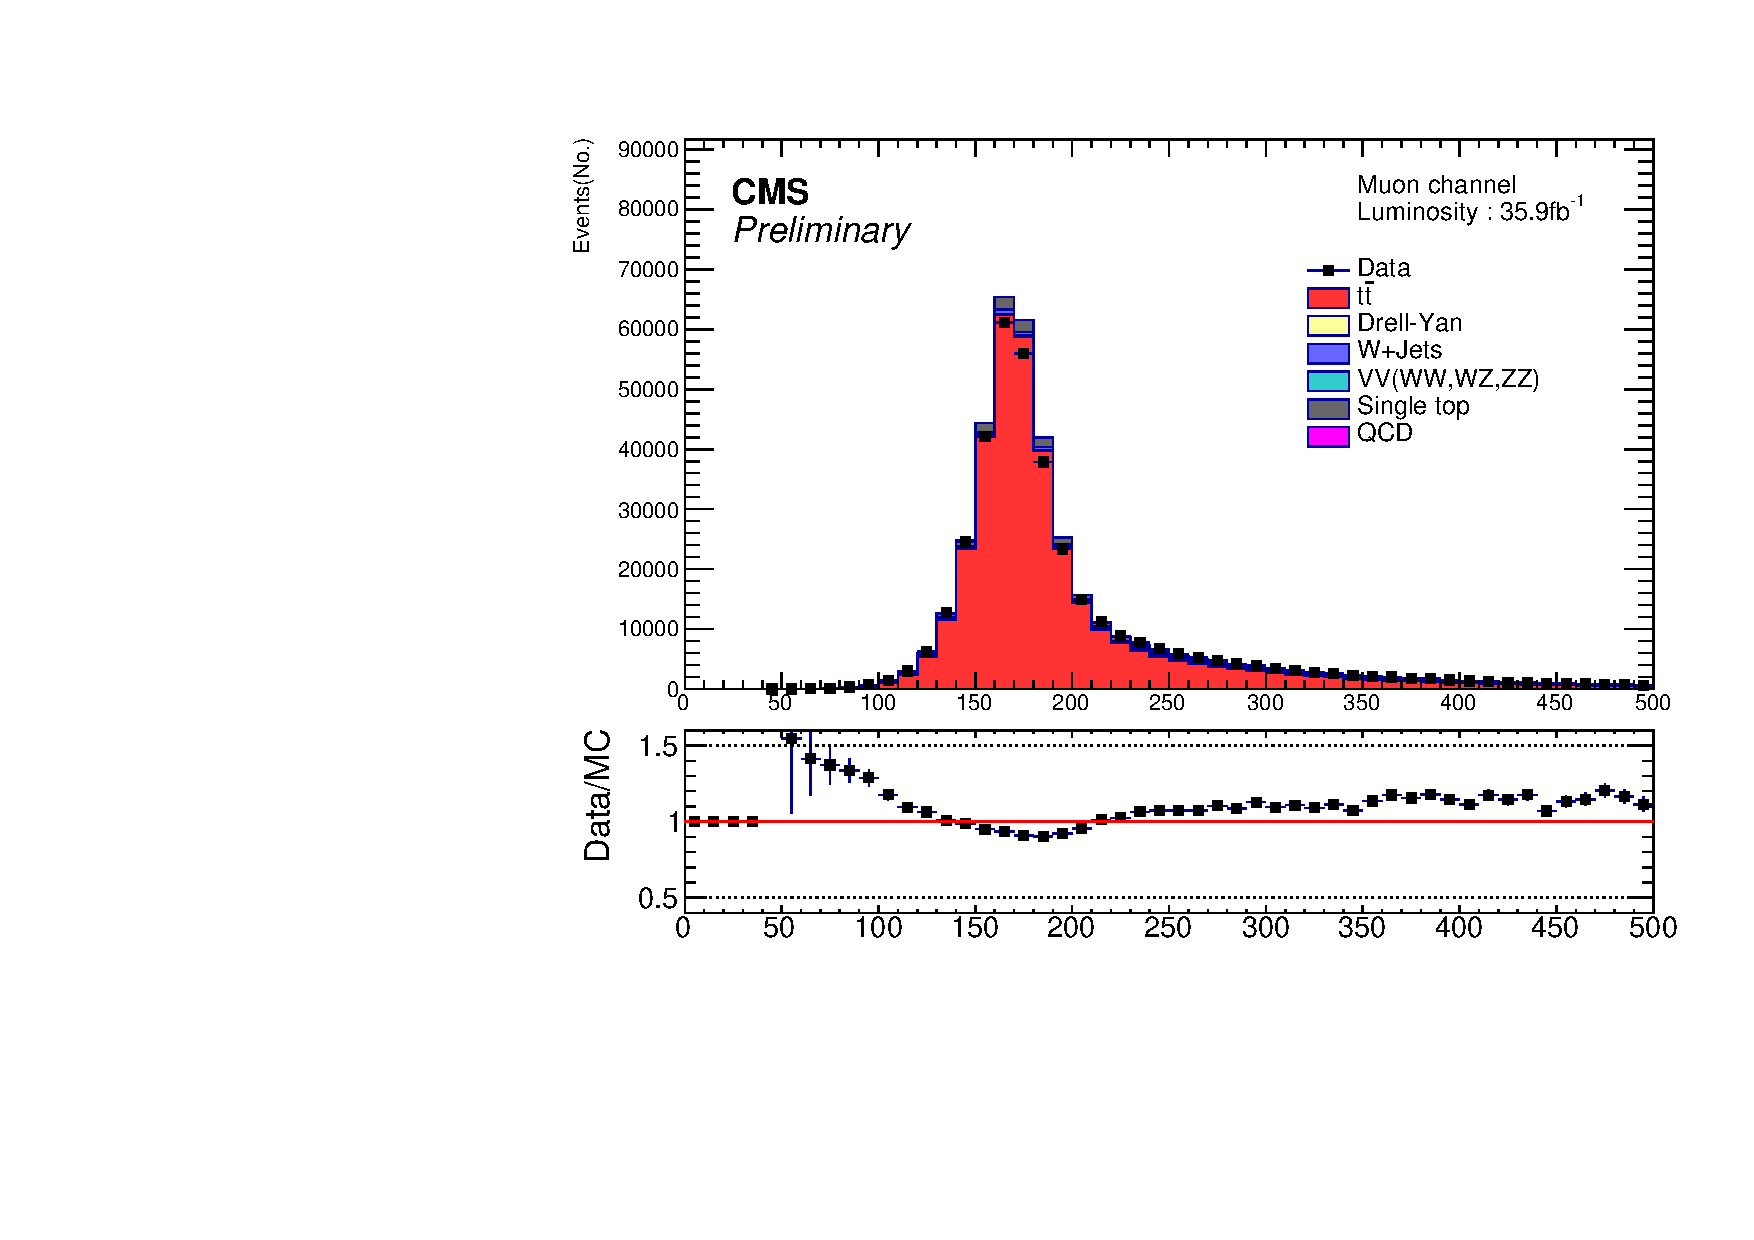
\includegraphics[width=0.45\textwidth]{Figures/EventSelReco/Mjjb/chi2_NC_long_HadTop_mu.pdf}}
    \subfigure[electron channel]{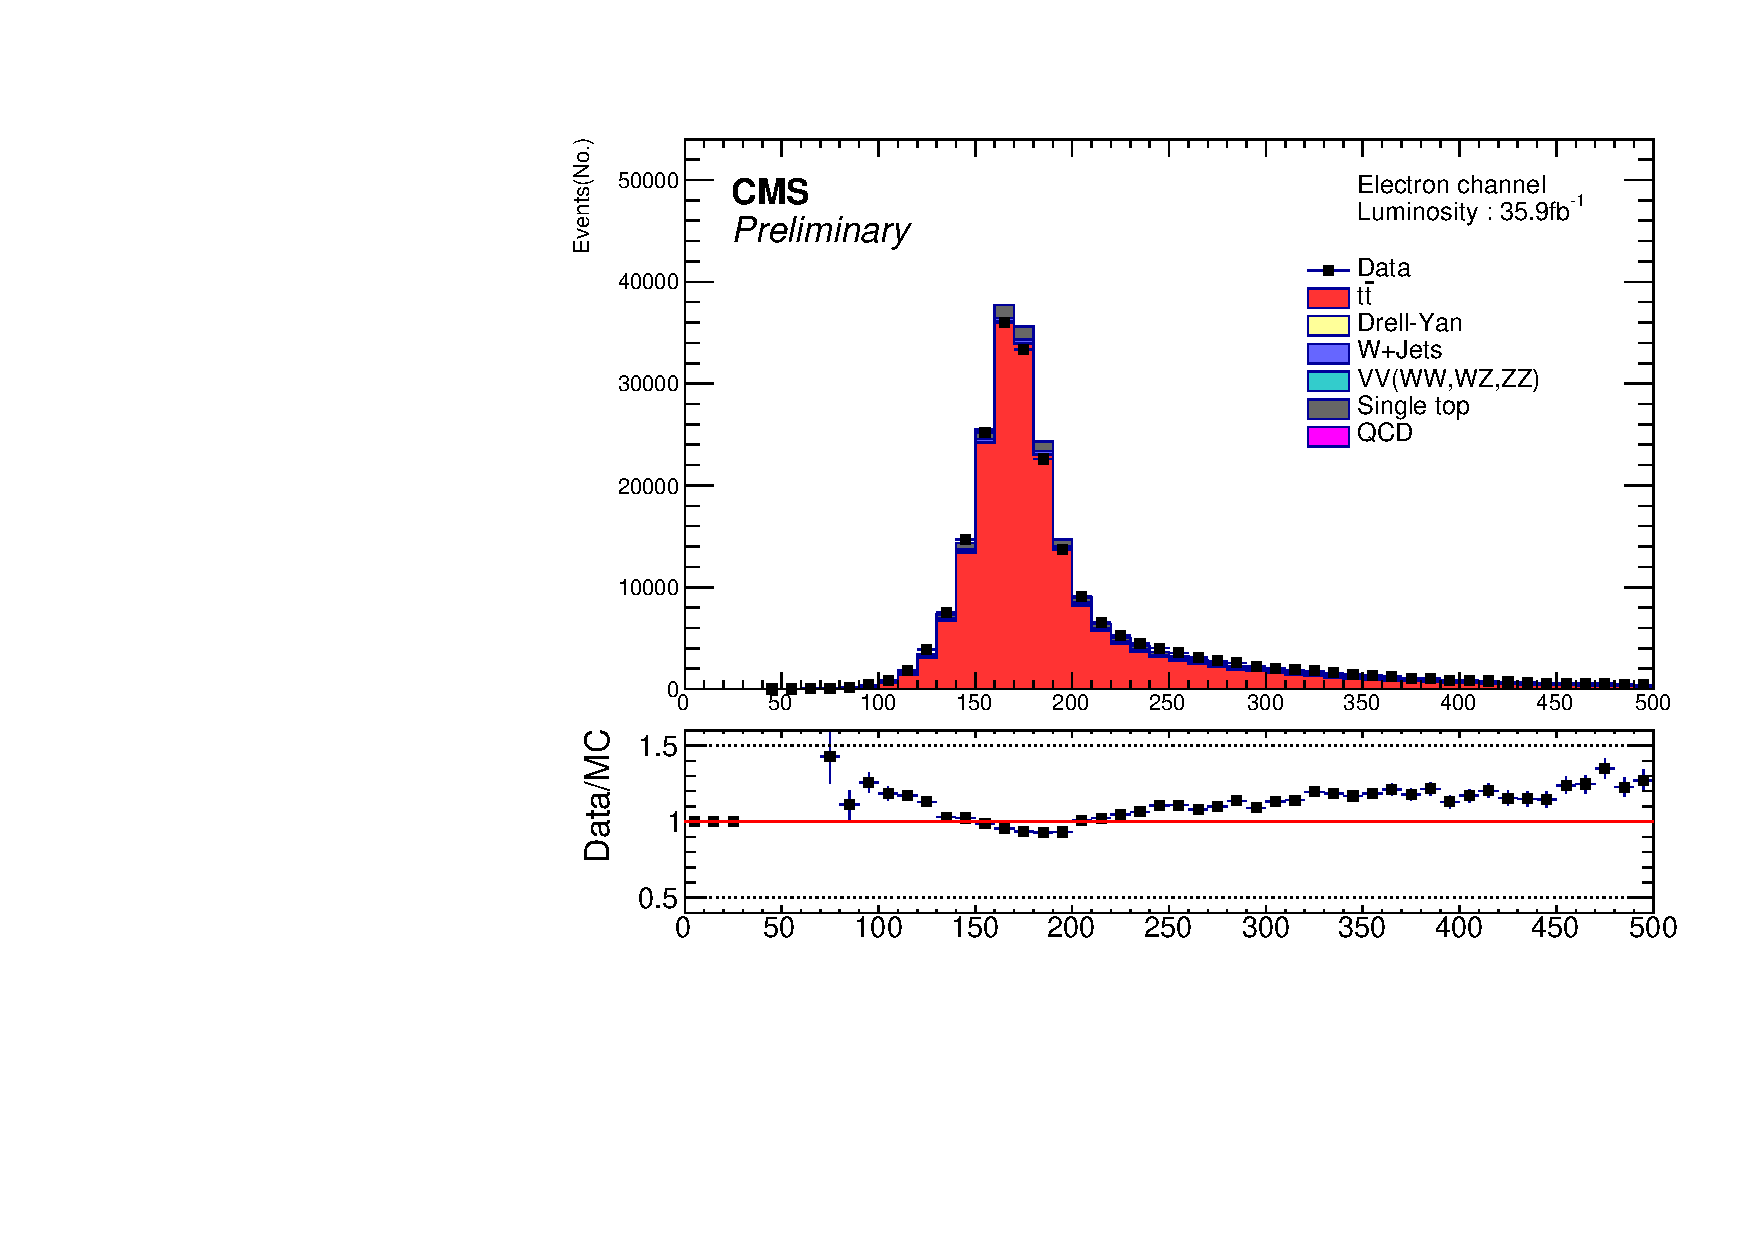
\includegraphics[width=0.45\textwidth]{Figures/EventSelReco/Mjjb/chi2_NC_long_HadTop_el.pdf}}\\
\caption{}
\label{EventSelReco:fig:chi2_SR_NC_Mjjb}
\end{figure}
\FloatBarrier

		\subsubsection{MVA Method}
		\label{sssec:mva_intro} 

			However, to improve the reconstruction performance in my analysis, there is another method - $\textbf{Multi-Variate Analysis (MVA)}$ can be adopted to do well in this reconstruction part. It has been not a common way to used in this step yet compared to signal and background samples' classification. In order to check the improvement between usual and new method, in the following rest analysis, the comparison of analysis results of $\chi^2_{min}$ method and MVA method will be shown simultaneously. 

			The concept of MVA is to use basic machine learning method to classify signal and background, we'll take advantage of MVA discriminating ability to improve the correctness rate of selection compared with $\chi^2_{min}$ method.
				
			As the usage of classification, one should define the "signal" and "background" in MVA configuration. In most particle physics analysis with MVA, $"$signal$"$ means the new physics which is expected to be discovered and the $"$background$"$ means samples from the other known physics. Different as usual, in this analysis,

			\begin{itemize}

				\item $\textbf{Sample}$ : signal simulation sample($t\bar{t}$ MC) with full event selection(\ref{ssec:EvtSel_SR})
				\item Randomly half for training sample, another half for testing sample
				\item In each event,
				\begin{enumerate}
					\item $\textbf{Signal}$ is recognized as the correct combination of objects hadronically decaying from t($\bar{t}$)-quark in an event
					\item $\textbf{Background}$ are all the other incorrect combinations in an event
				\end{enumerate}
			\end{itemize}

			To identify whether one combination is the 2 jets and the correct detector-level's objects from generator-level's particles, the $\Delta R$ method is used to match them. The matching method is to compare the angle distribution between detector-level objects and generator-level particles with $\Delta R$ < 0.4. 
			
			\begin{equation}
			\Delta R = \sqrt{ (\eta_{det} - \eta_{gen})^2 - (\phi_{det} - \phi_{gen})^2 } < 0.4
			\label{eq:gen_matching}
			\end{equation}
		
			With concept of machine learning, we need to train with informations of classes( $"$signal$"$ and $"$backgroud$"$ in this case ) and get out an algorithm to make distinguishment. Following the original $\chi^2_{min}$ method's variables, we started MVA with inputting 2 variables : $m_{jj}$, $m_{jjb}$, as informations to be used for distinguishment. There are three machine learning methods I used for testing: $\textbf{MLP}$(ANN, Artificial Neuro-Network), $\textbf{BDT}$(Boosted Decision Tree), $\textbf{BDTG}$(Boosted Decision Tree Gradient). 

			The training result shows below:

\begin{figure}[H]
\centering
	\subfigure[BDT's separation result]{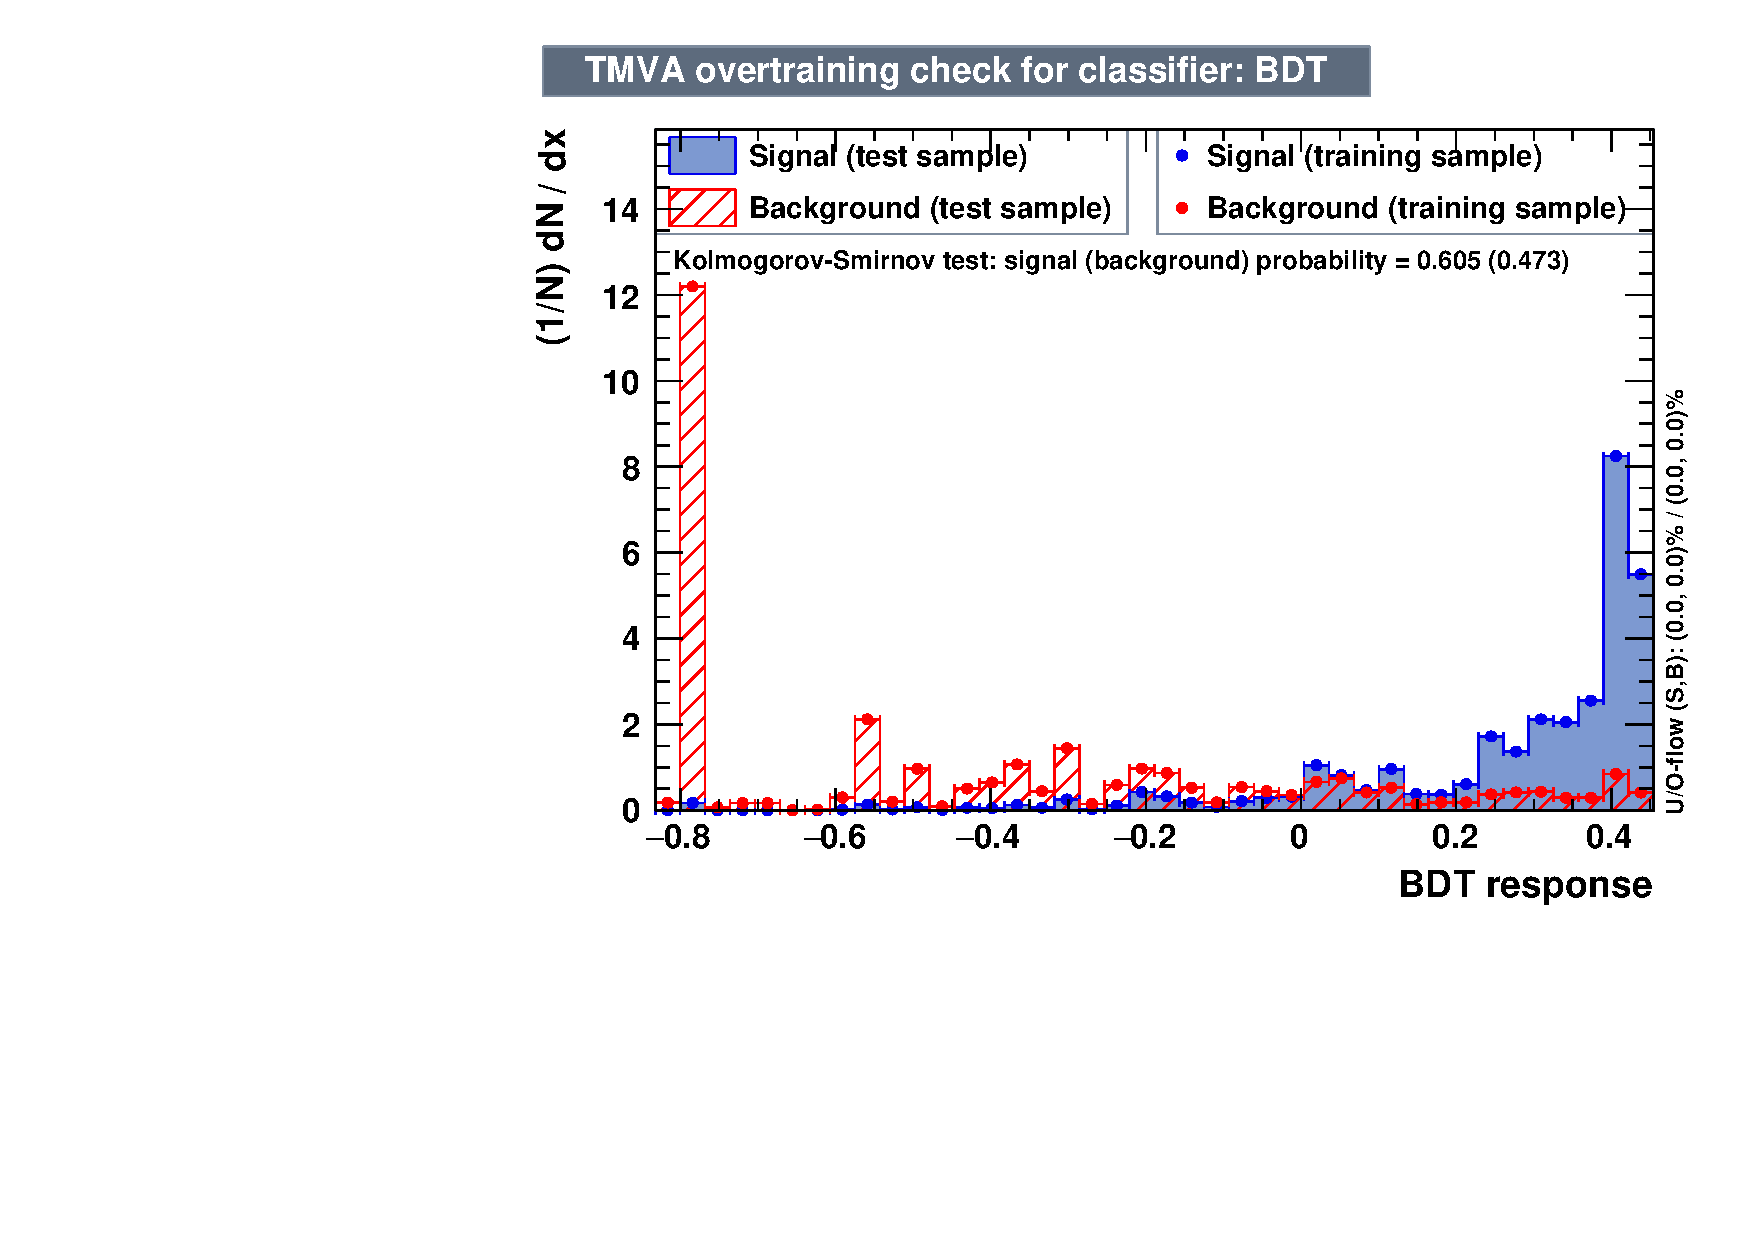
\includegraphics[width=0.45\textwidth]{Figures/EventSelReco/a04_all_BDT_sep.pdf}}
    \subfigure[BDTG's separation result]{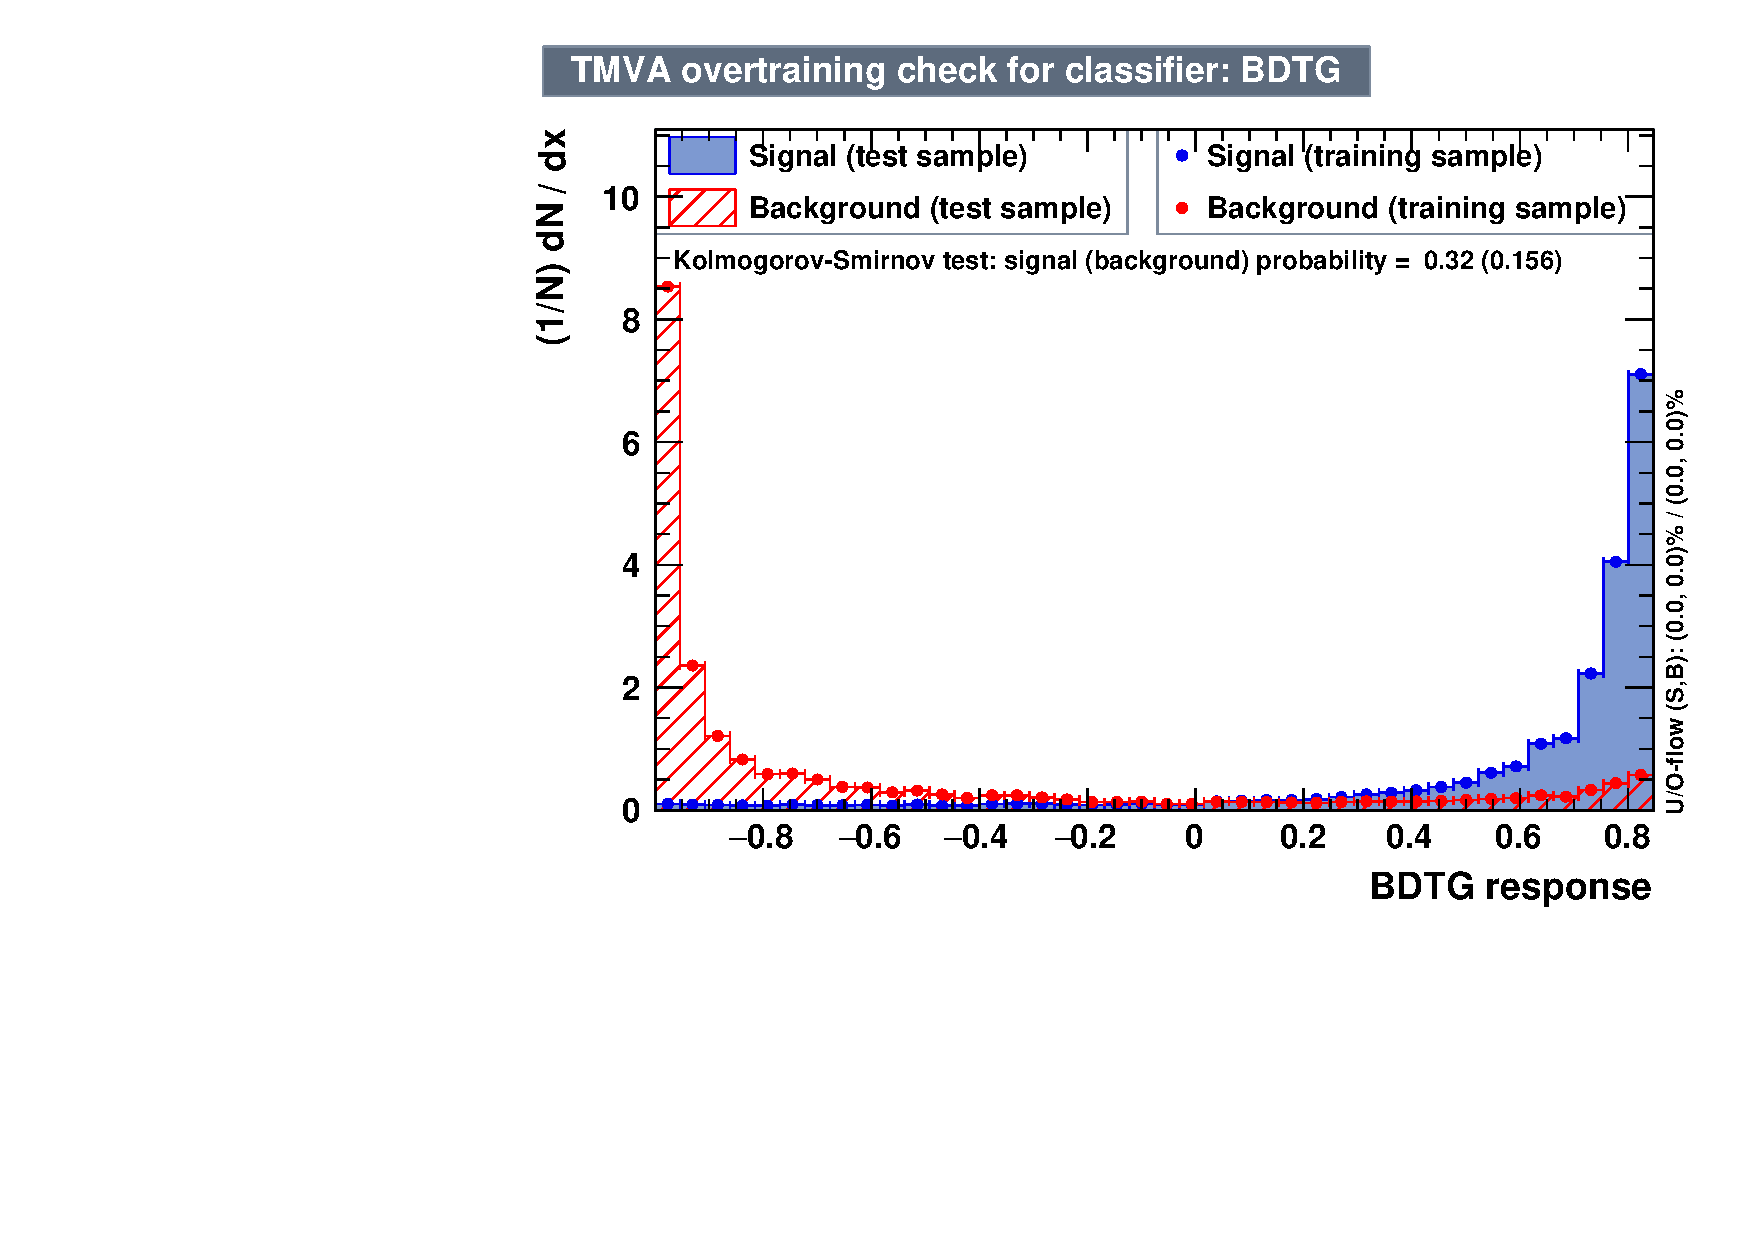
\includegraphics[width=0.45\textwidth]{Figures/EventSelReco/a04_all_BDTG_sep.pdf}}\\
    \subfigure[MLP's separation result]{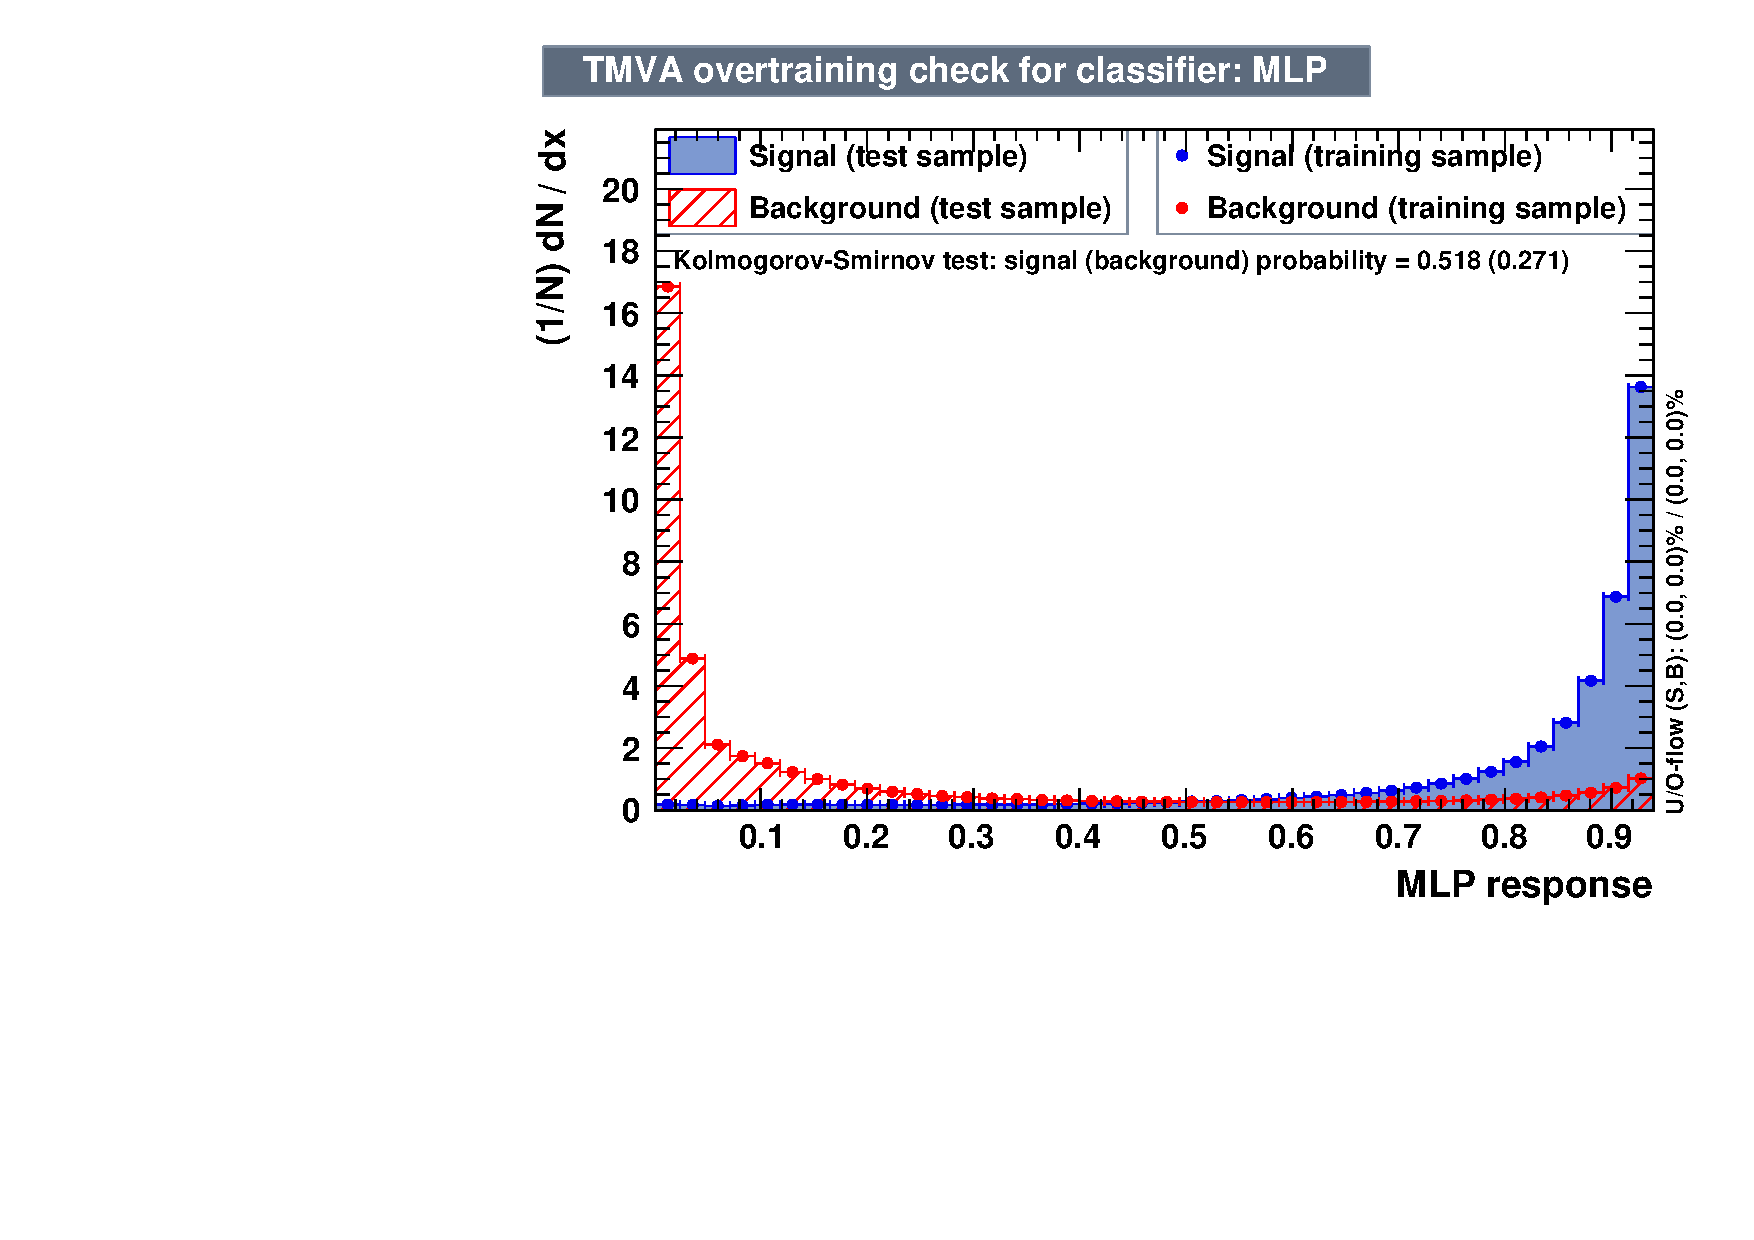
\includegraphics[width=0.45\textwidth]{Figures/EventSelReco/a04_all_MLP_sep.pdf}}\\
\caption{The seperating distribution on signal and background}
\label{EventSelReco:fig:Sep_a04}
\end{figure}
\FloatBarrier

			The separation plots Fig.\ref{EventSelReco:fig:Sep_a04} shows the machine learning methods' separating ability. The distributions in these plots are the seperation performance between $"$signal$"$ and $"$background$"$(right and wrong objects combination) under training sample and testing sample with given machine learning method. As we can see that if we want to pick out $"$signal$"$(right combination), just choose the jjb combination who has the higher MVA score as the right one.

\begin{figure}[H]
\centering{}
    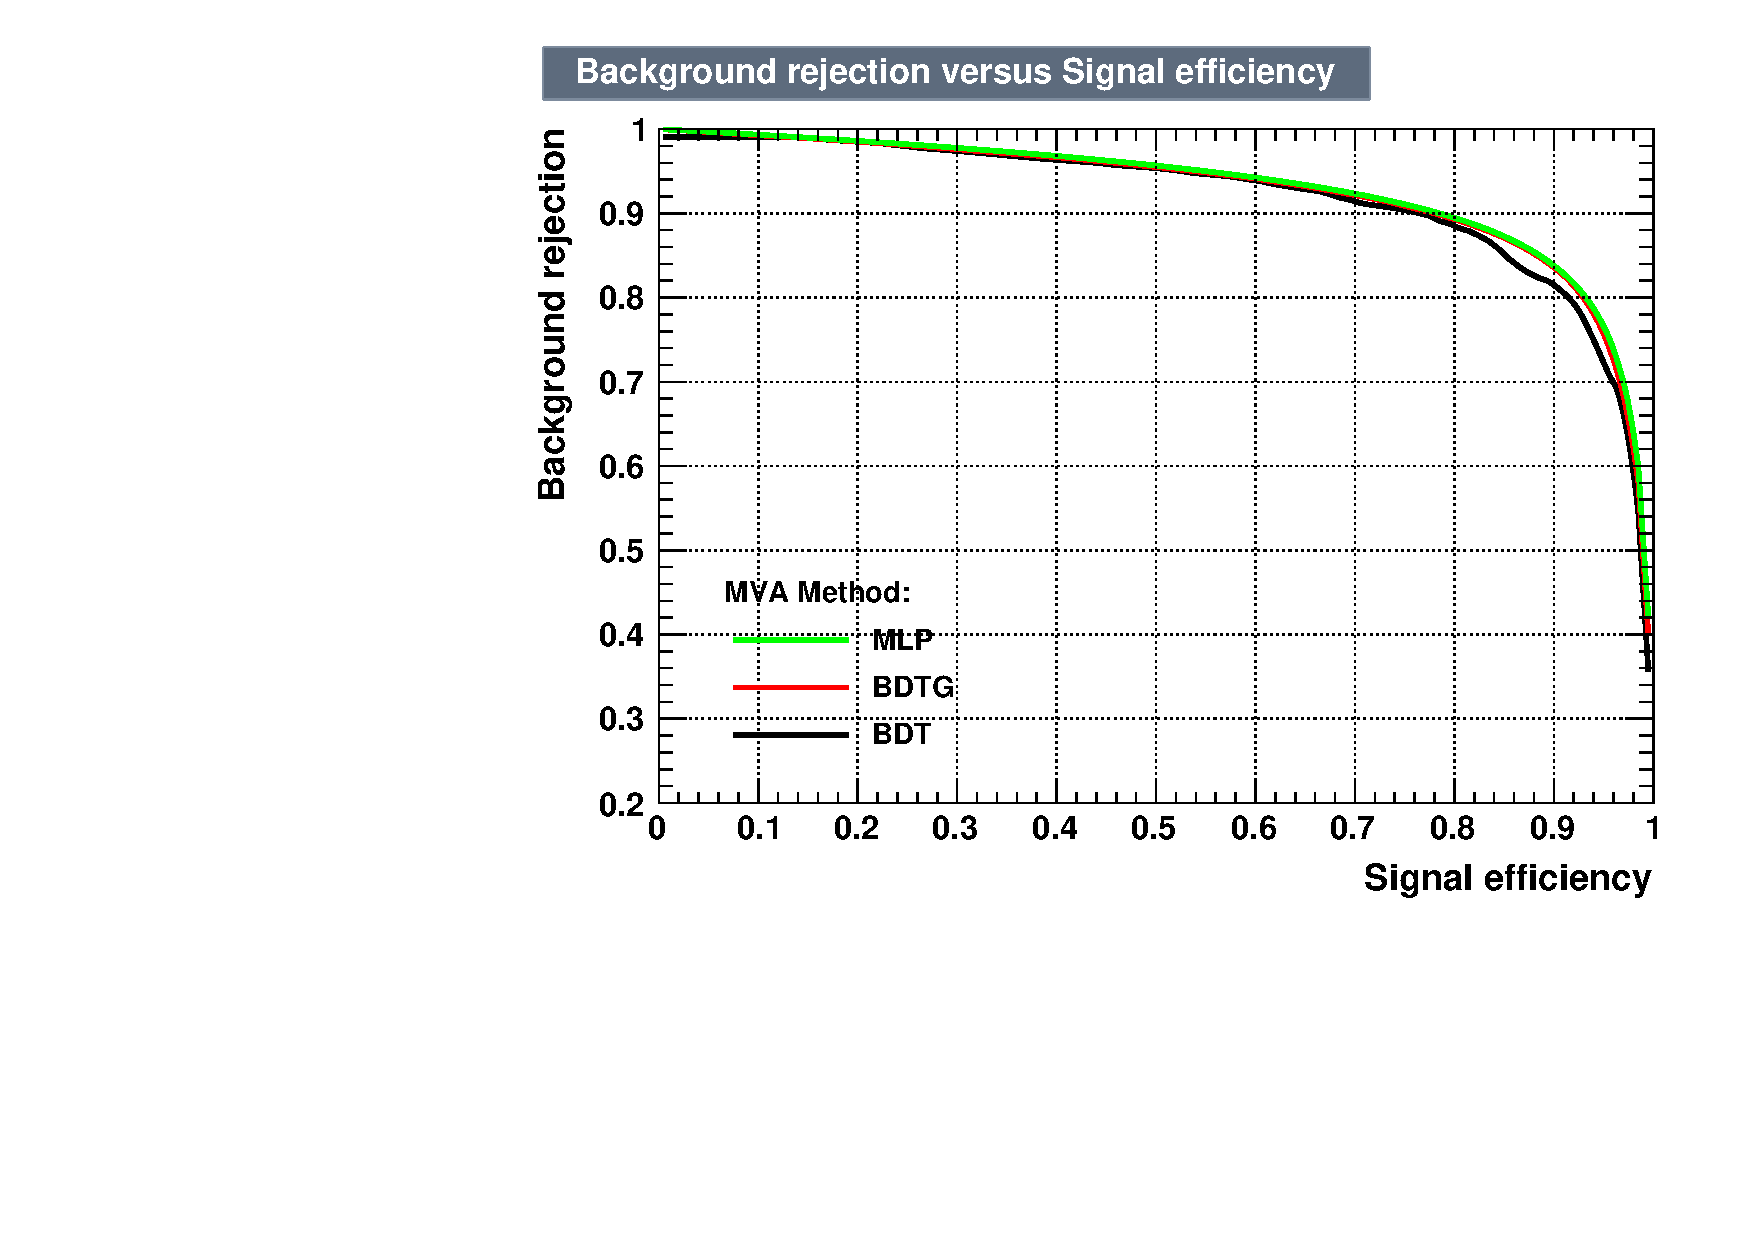
\includegraphics[width=0.6\textwidth]{Figures/EventSelReco/a04_all_ROC.pdf}\\
\caption{Receiver Operating Characteristic(ROC) curve of various machine learning method}
\label{EventSelReco:fig:ROC_a04}
\end{figure}
\FloatBarrier
	
			The $\textbf{Receiver Operating Characteristic(ROC)}$ curve plot Fig.\ref{EventSelReco:fig:ROC_a04} can tell if it's given a cut on the output MVA score in separation distribution Fig.\ref{EventSelReco:fig:Sep_a04} to extract the $"$signal$"$, how the background rejection ratio vary when signal efficiency change. It can be infered that, the good performance is that when one rejects more ratio of background and at the same time reserves more ratio of signal(high signal efficiency). In other words, the bigger area under the ROC curve, the better the method is. However, the previous ROC criterion are just available and meaningful for the common case - one use MVA to separate the 2 different physics sample which are independent to each other, for example, use MVA to separate sigle $t$ and $t\bar{t}$ sample. In this analysis case, the signal and background are not separate like that kind in common. Being not independent 2 samples, signal and background are at the same time in one event instead. There are couple of complicated correlation between them. Therefore, the separation and ROC plots are not really fair anymore. As they going to not to be relative directly, there must be a standard to tell how MVA perform(That is the $b\bar{b}$ separation in \ref{ssec:bbsep}).

			And also, it is better to use MVA with more variables than just $m_{jj}$ and $m_{jjb}$. There are 3 variables sets after a bunch of trials here to input and train. It's a remindful item that they are the variables of each combination in any event.

			\begin{enumerate}
			\item The first set: (2 variables)
				\begin{itemize}
				\item $m_{jjb}$, $m_{jj}$
				\end{itemize}

			%%% TODO: this set need to be eliminate before showing the result of bbsep performance
			\item The second set: (8 variables)
				\begin{itemize}
				\item $m_{jjb}$, $m_{jj}$
				\item 2 jets'(jj) $\emph{sum of}$ $P_{T}$, $\Delta \phi$, $\Delta \eta$
				\item selected lepton and leptonic b-jet's $\emph{sum of}$ $P_{T}$, $\Delta \phi$, $\Delta \eta$ 
				\end{itemize}

			\item The third set: (20 variables)
				\begin{itemize}
				\item $m_{jjb}$, $m_{jj}$
				\item 2 jets'(jj) $\emph{sum of}$ $P_{T}$, $|\Delta P_{T}|$, $\Delta R$
				\item hadronic W(j+j) and hadronic b-jet's $\emph{sum of}$ $P_{T}$, $|\Delta P_{T}|$, $\Delta R$
				\item selected lepton and hadronic b-jet's $\emph{sum of}$ $P_{T}$, $|\Delta P_{T}|$, $\Delta R$
				\item selected lepton and hadronic W(j+j)'s $\emph{sum of}$ $P_{T}$, $|\Delta P_{T}|$, $\Delta R$
				\item hadronic W(j+j) and MET's $\emph{sum of}$ $P_{T}$, $|\Delta P_{T}|$, $\Delta \phi$
				\item hadronic b-jet and MET's $\emph{sum of}$ $P_{T}$, $|\Delta P_{T}|$, $\Delta \phi$
				\end{itemize}
			\end{enumerate}

			Besides the training result of the 2 variables' set have been shown(Fig.\ref{EventSelReco:fig:Sep_a04}, Fig.\ref{EventSelReco:fig:ROC_a04}), there are also the training results of 8 variables and 20 variables' cases:

			\begin{figure}[H]
			\centering
				\subfigure[BDT's separation result]{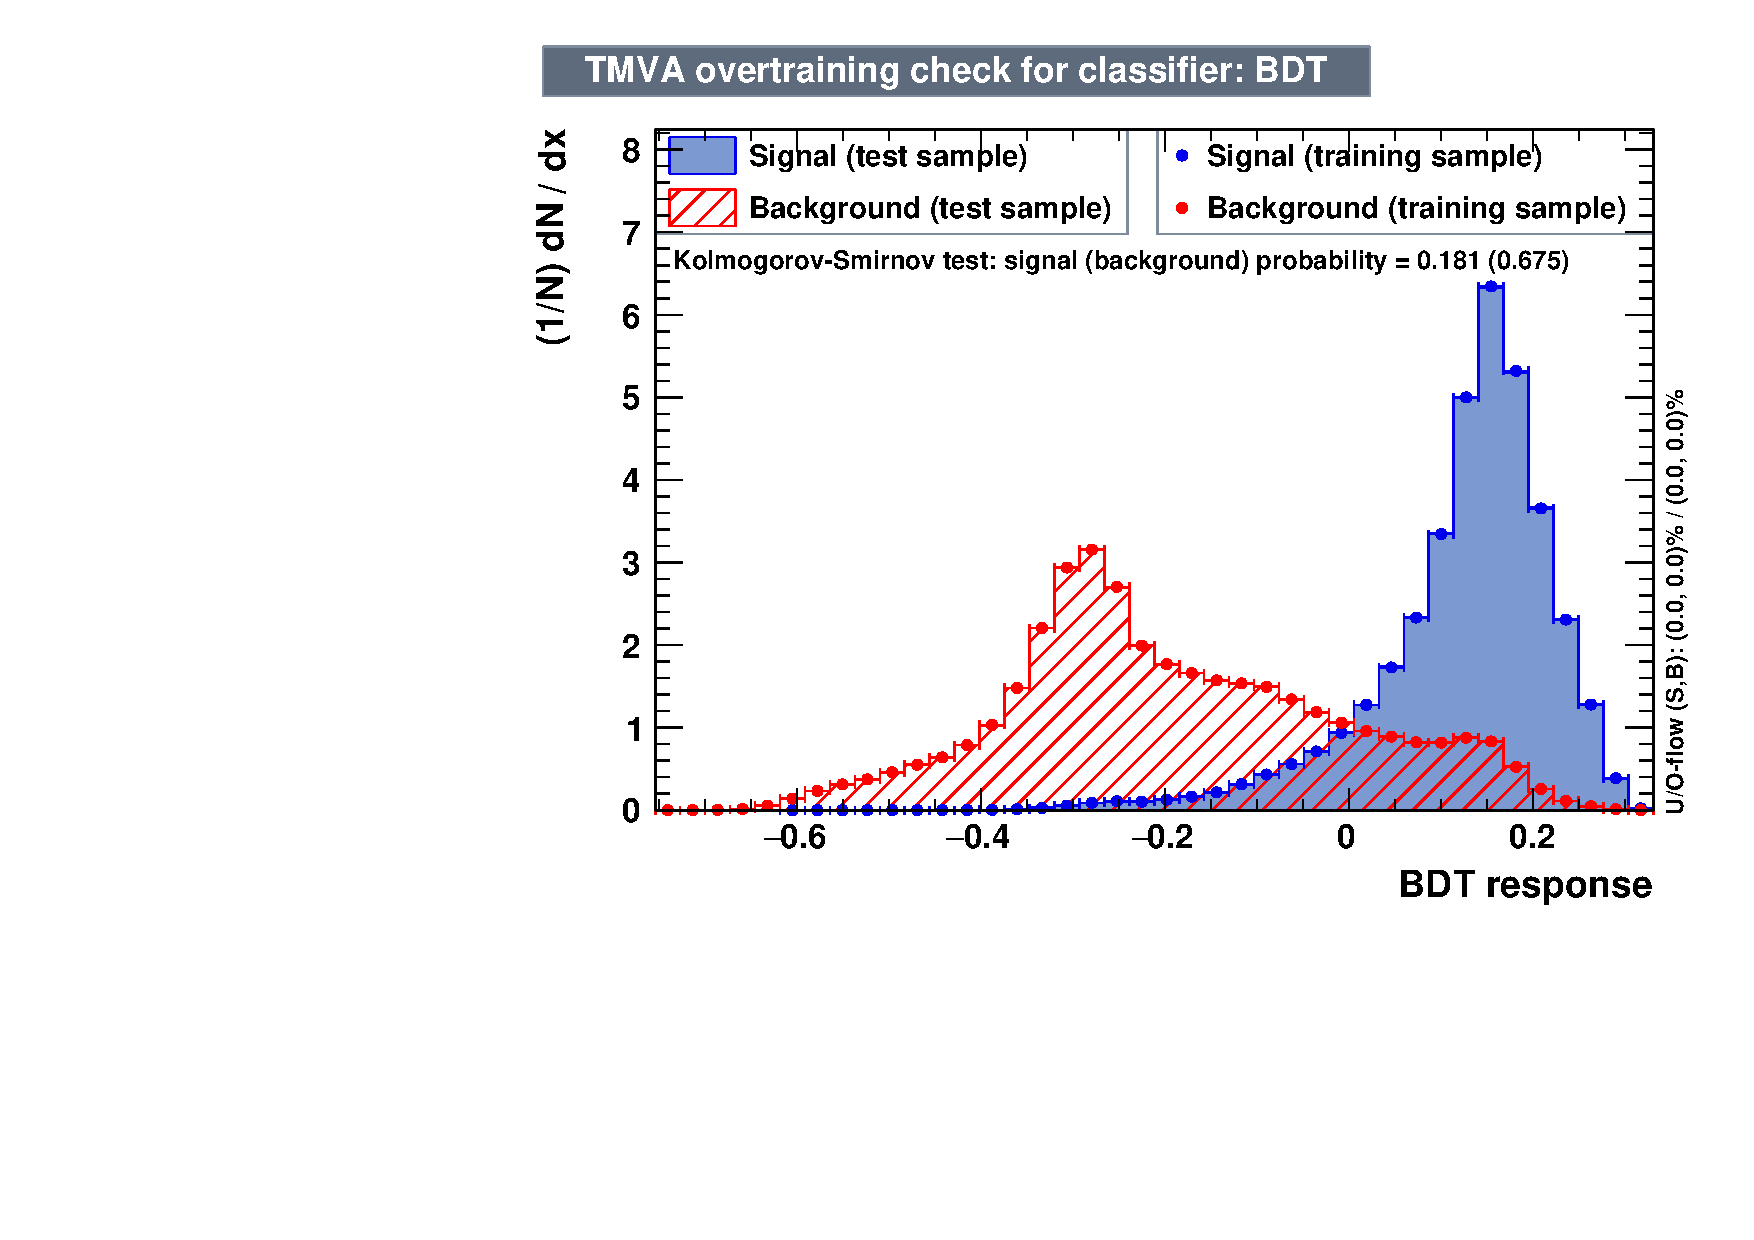
\includegraphics[width=0.45\textwidth]{Figures/EventSelReco/t13_BDT_sep.pdf}}
			    \subfigure[BDTG's separation result]{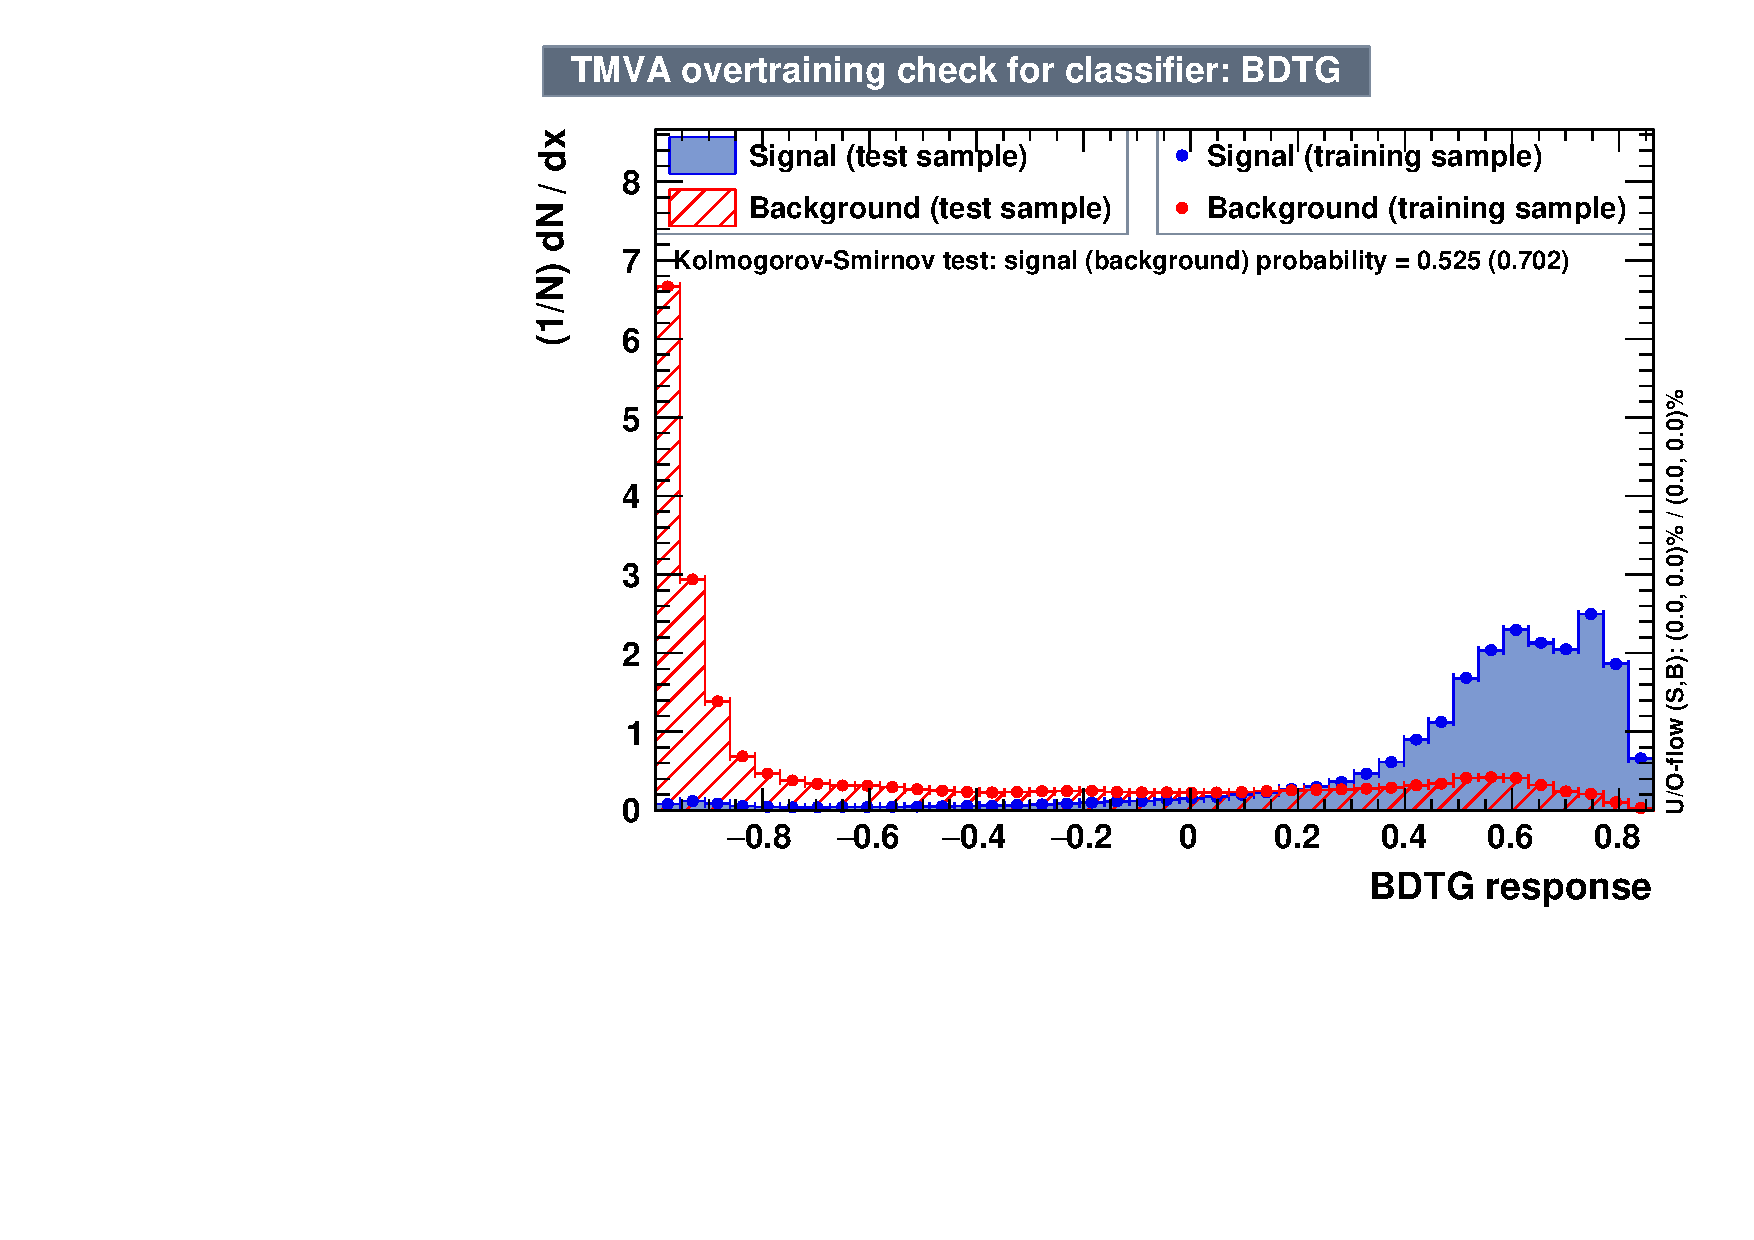
\includegraphics[width=0.45\textwidth]{Figures/EventSelReco/t13_BDTG_sep.pdf}}\\
			    \subfigure[MLP's separation result]{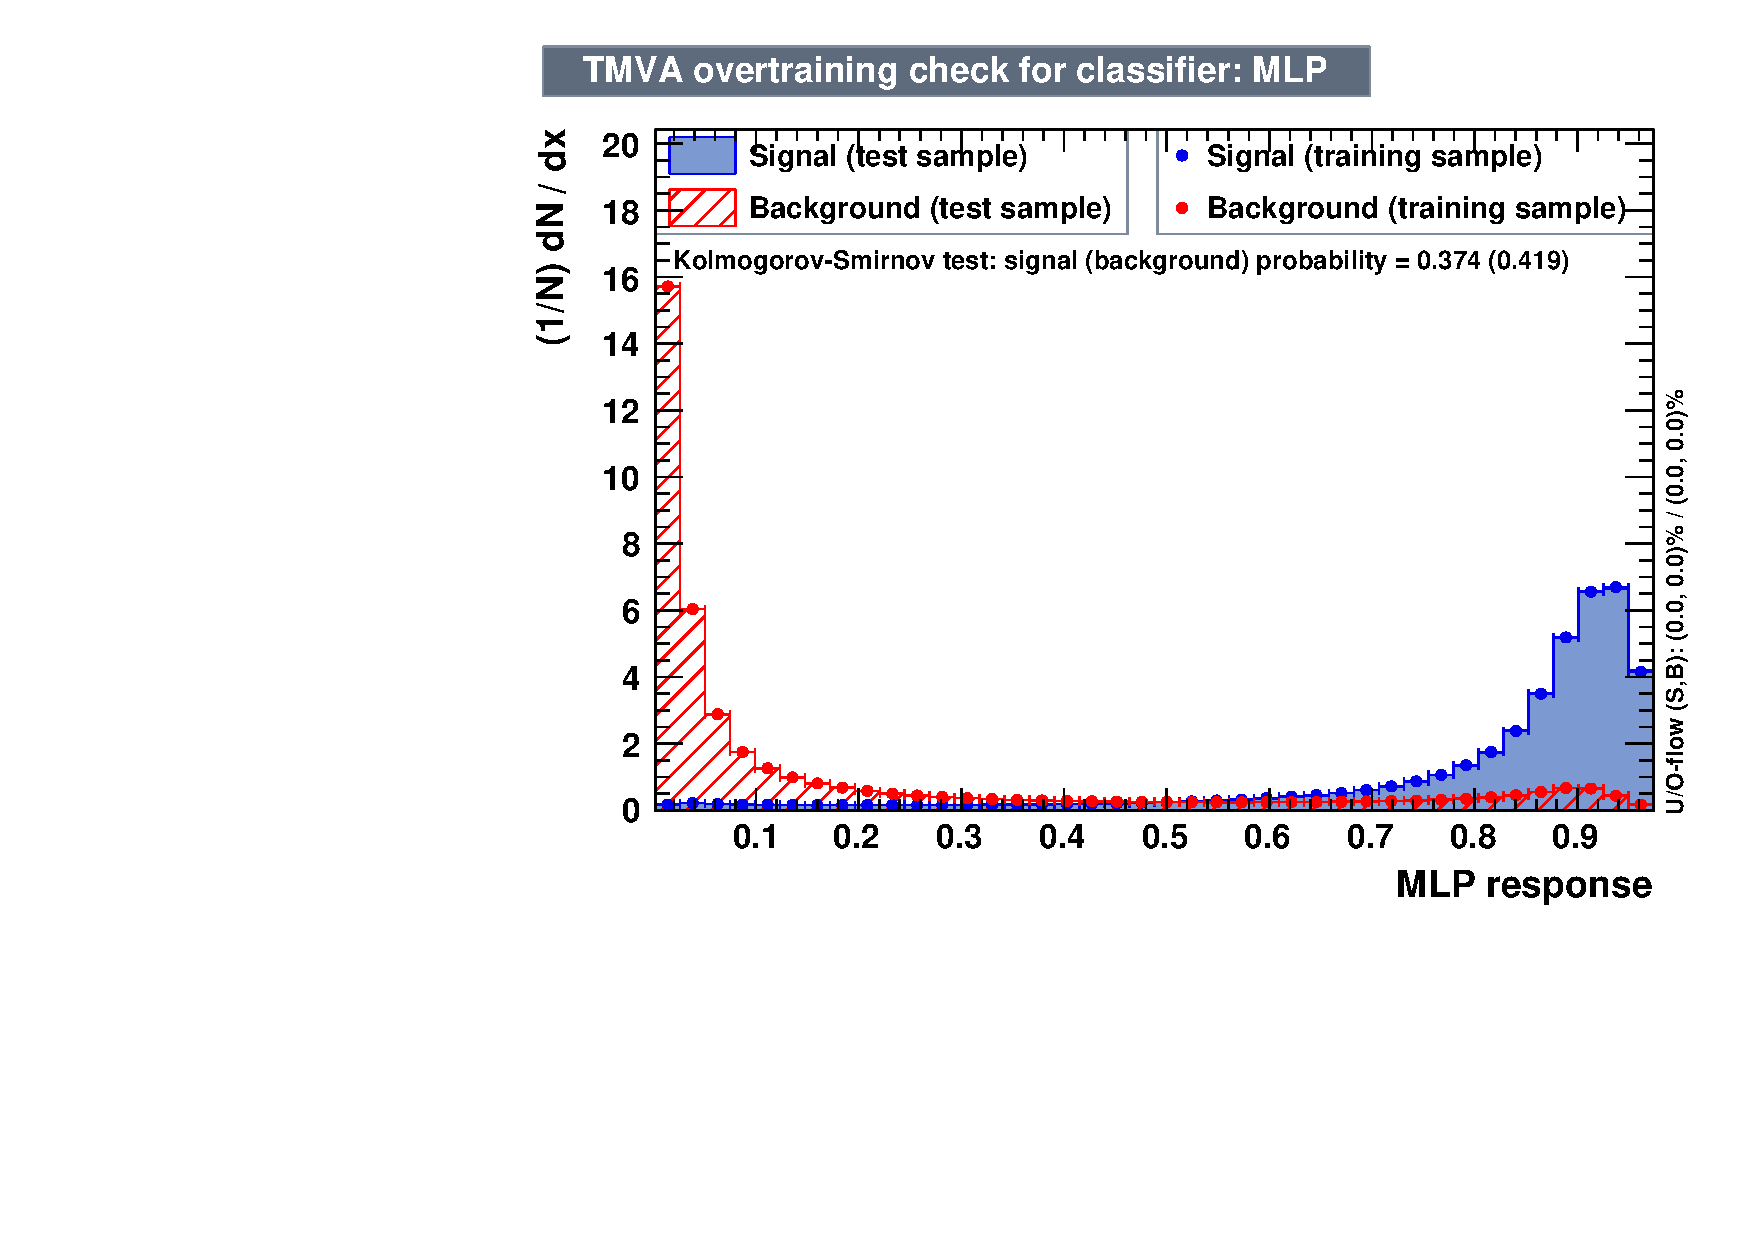
\includegraphics[width=0.45\textwidth]{Figures/EventSelReco/t13_MLP_sep.pdf}}
			    \subfigure[ROC curve]{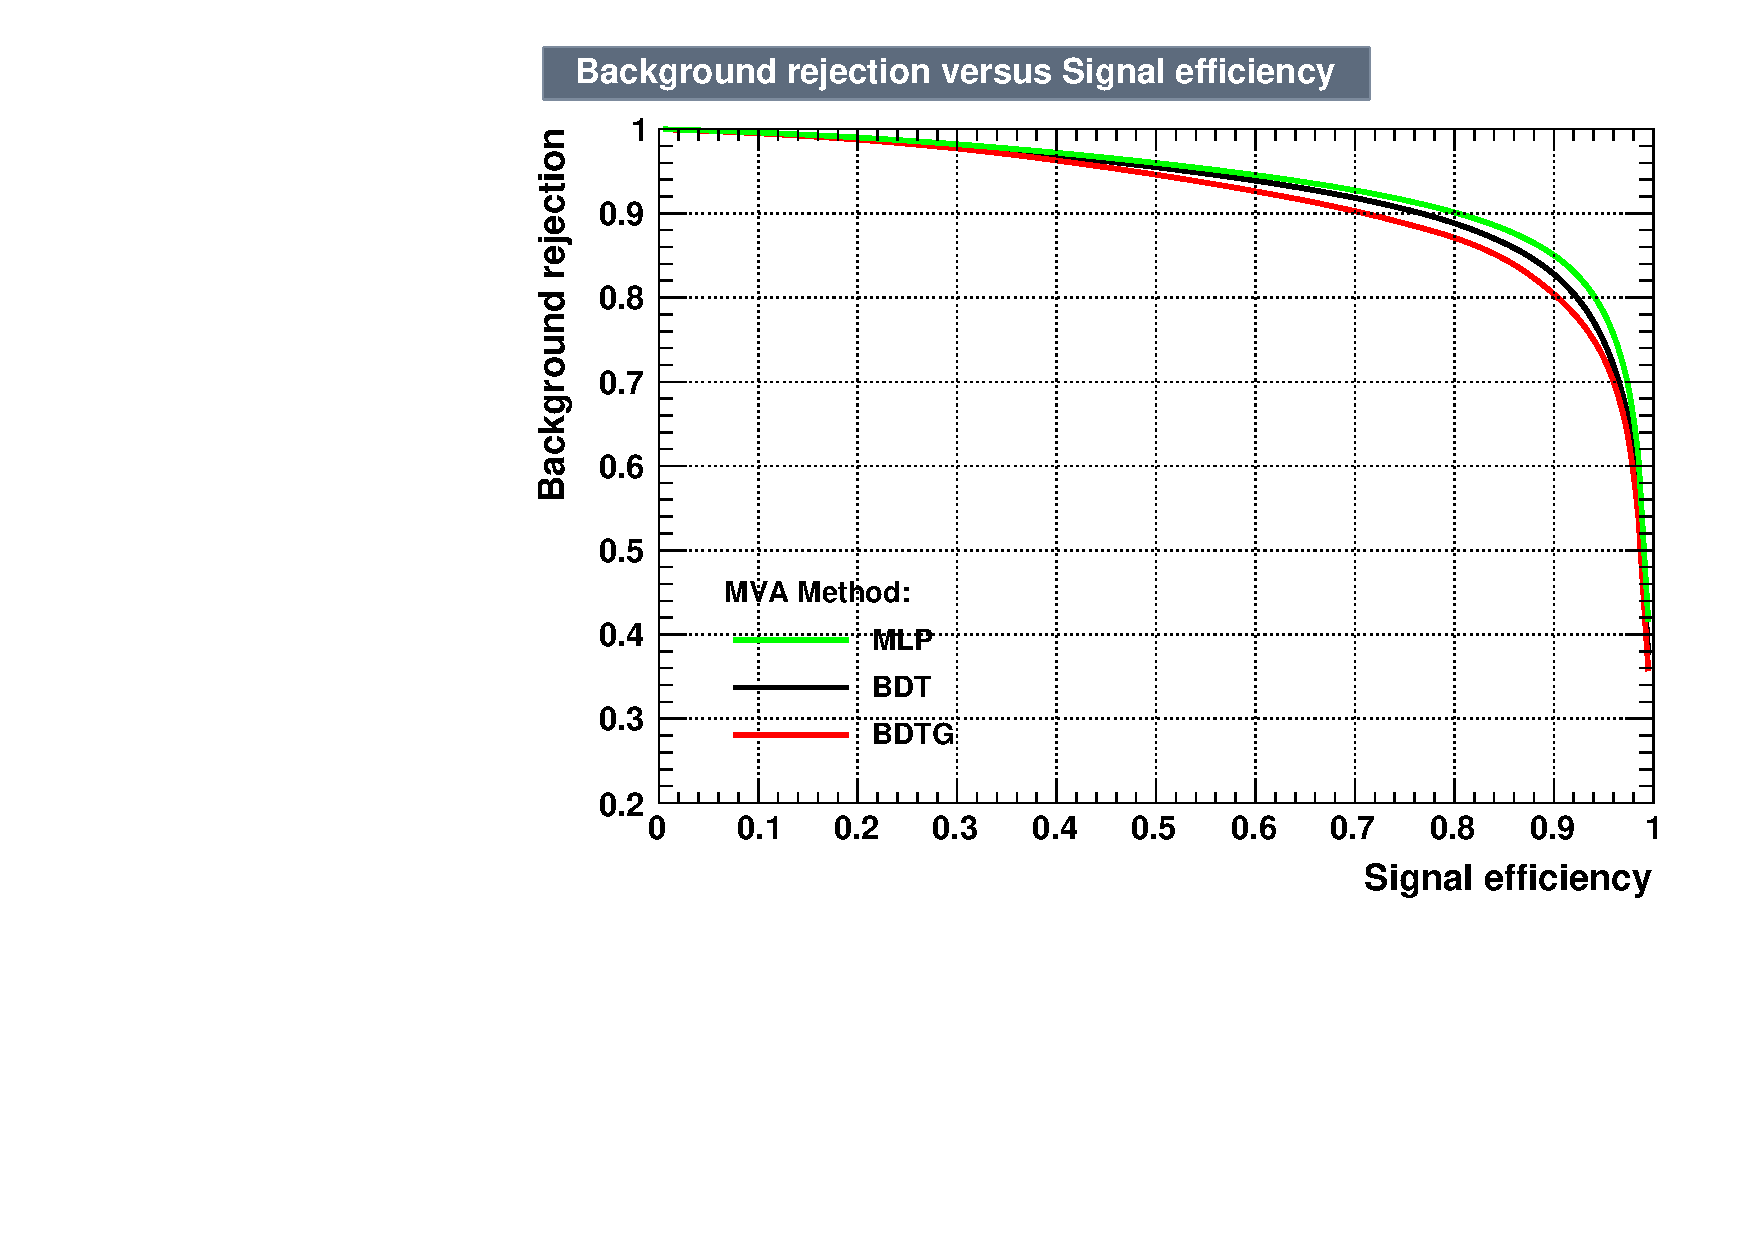
\includegraphics[width=0.45\textwidth]{Figures/EventSelReco/t13_ROC.pdf}}\\
			\caption{The training result of 8 variables set}
			\label{EventSelReco:fig:Sep_ROC_t13}
			\end{figure}
			\FloatBarrier

			\begin{figure}[H]
			\centering
				\subfigure[BDT's separation result]{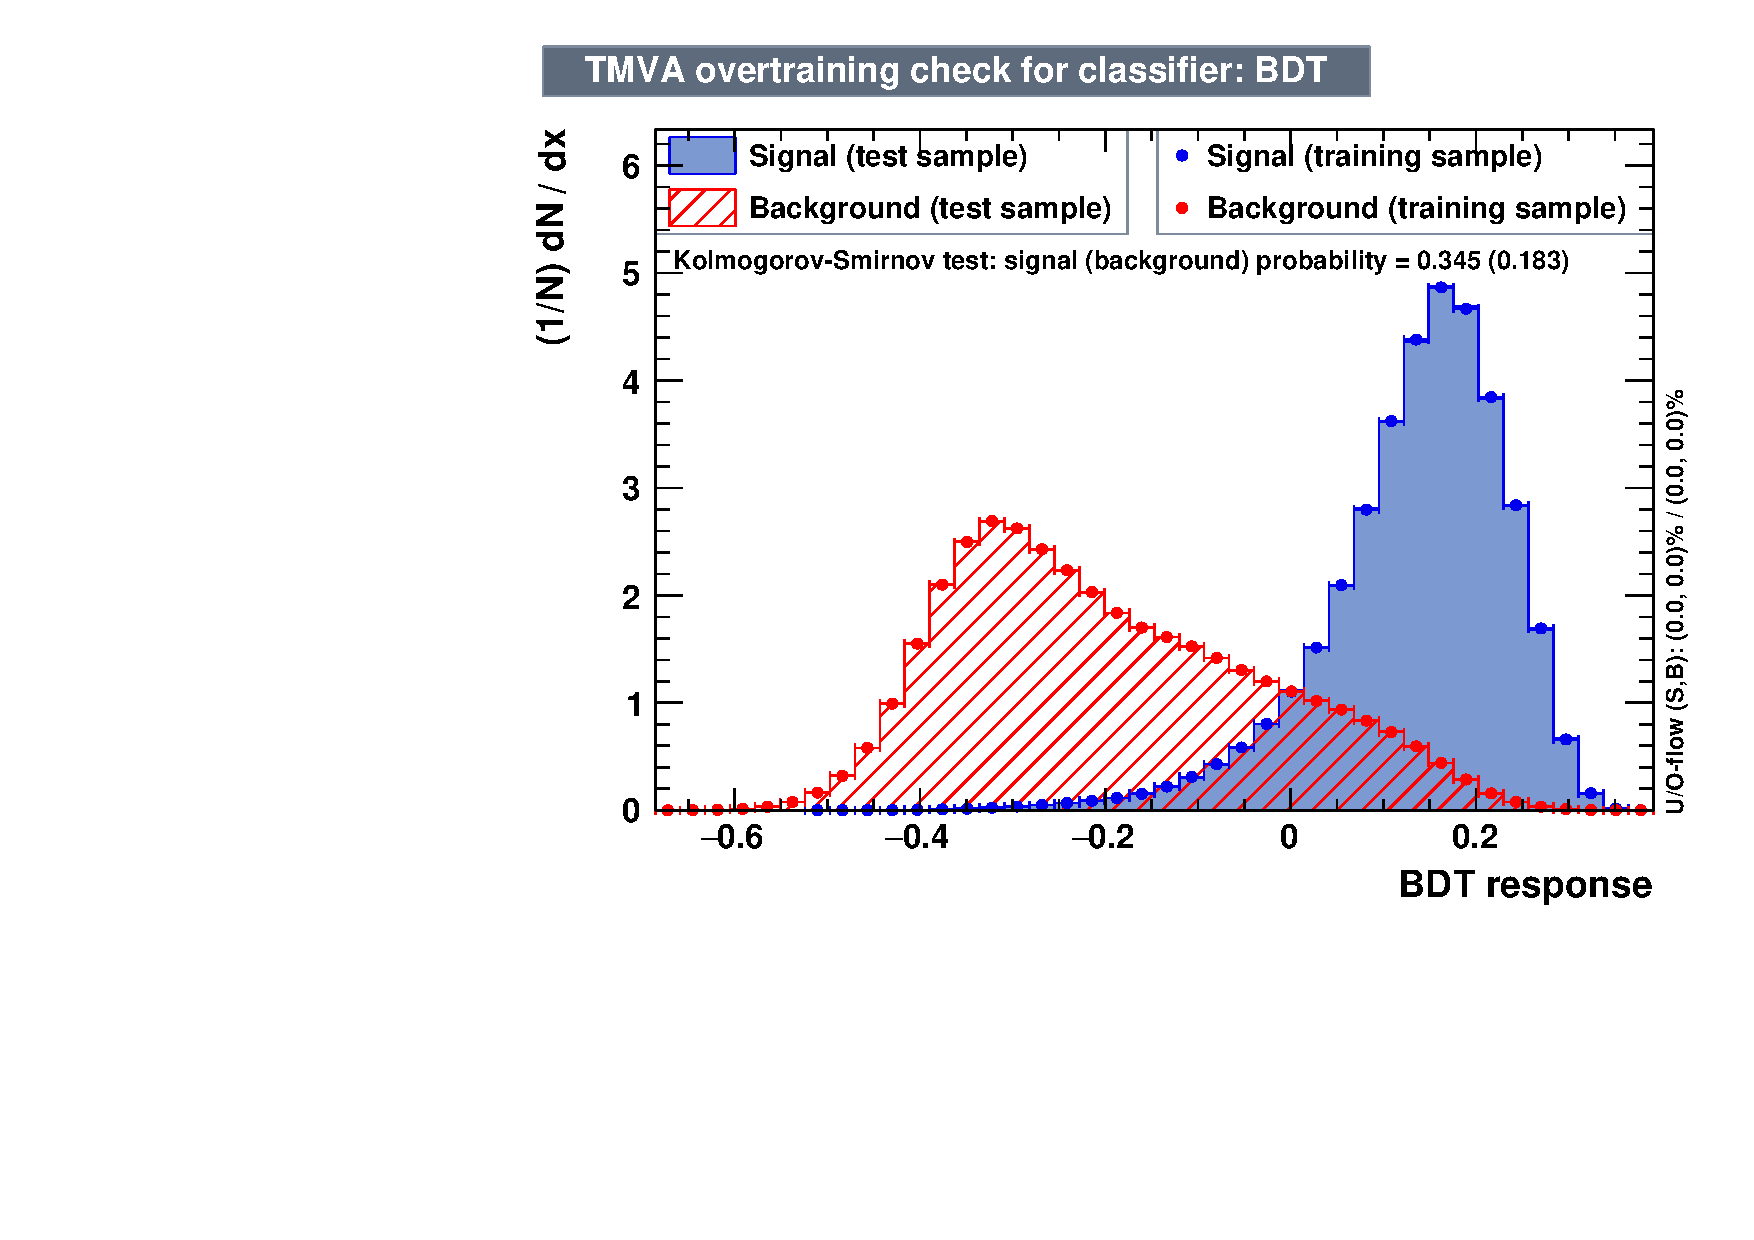
\includegraphics[width=0.45\textwidth]{Figures/EventSelReco/a05_all_BDT_sep.pdf}}
			    \subfigure[BDTG's separation result]{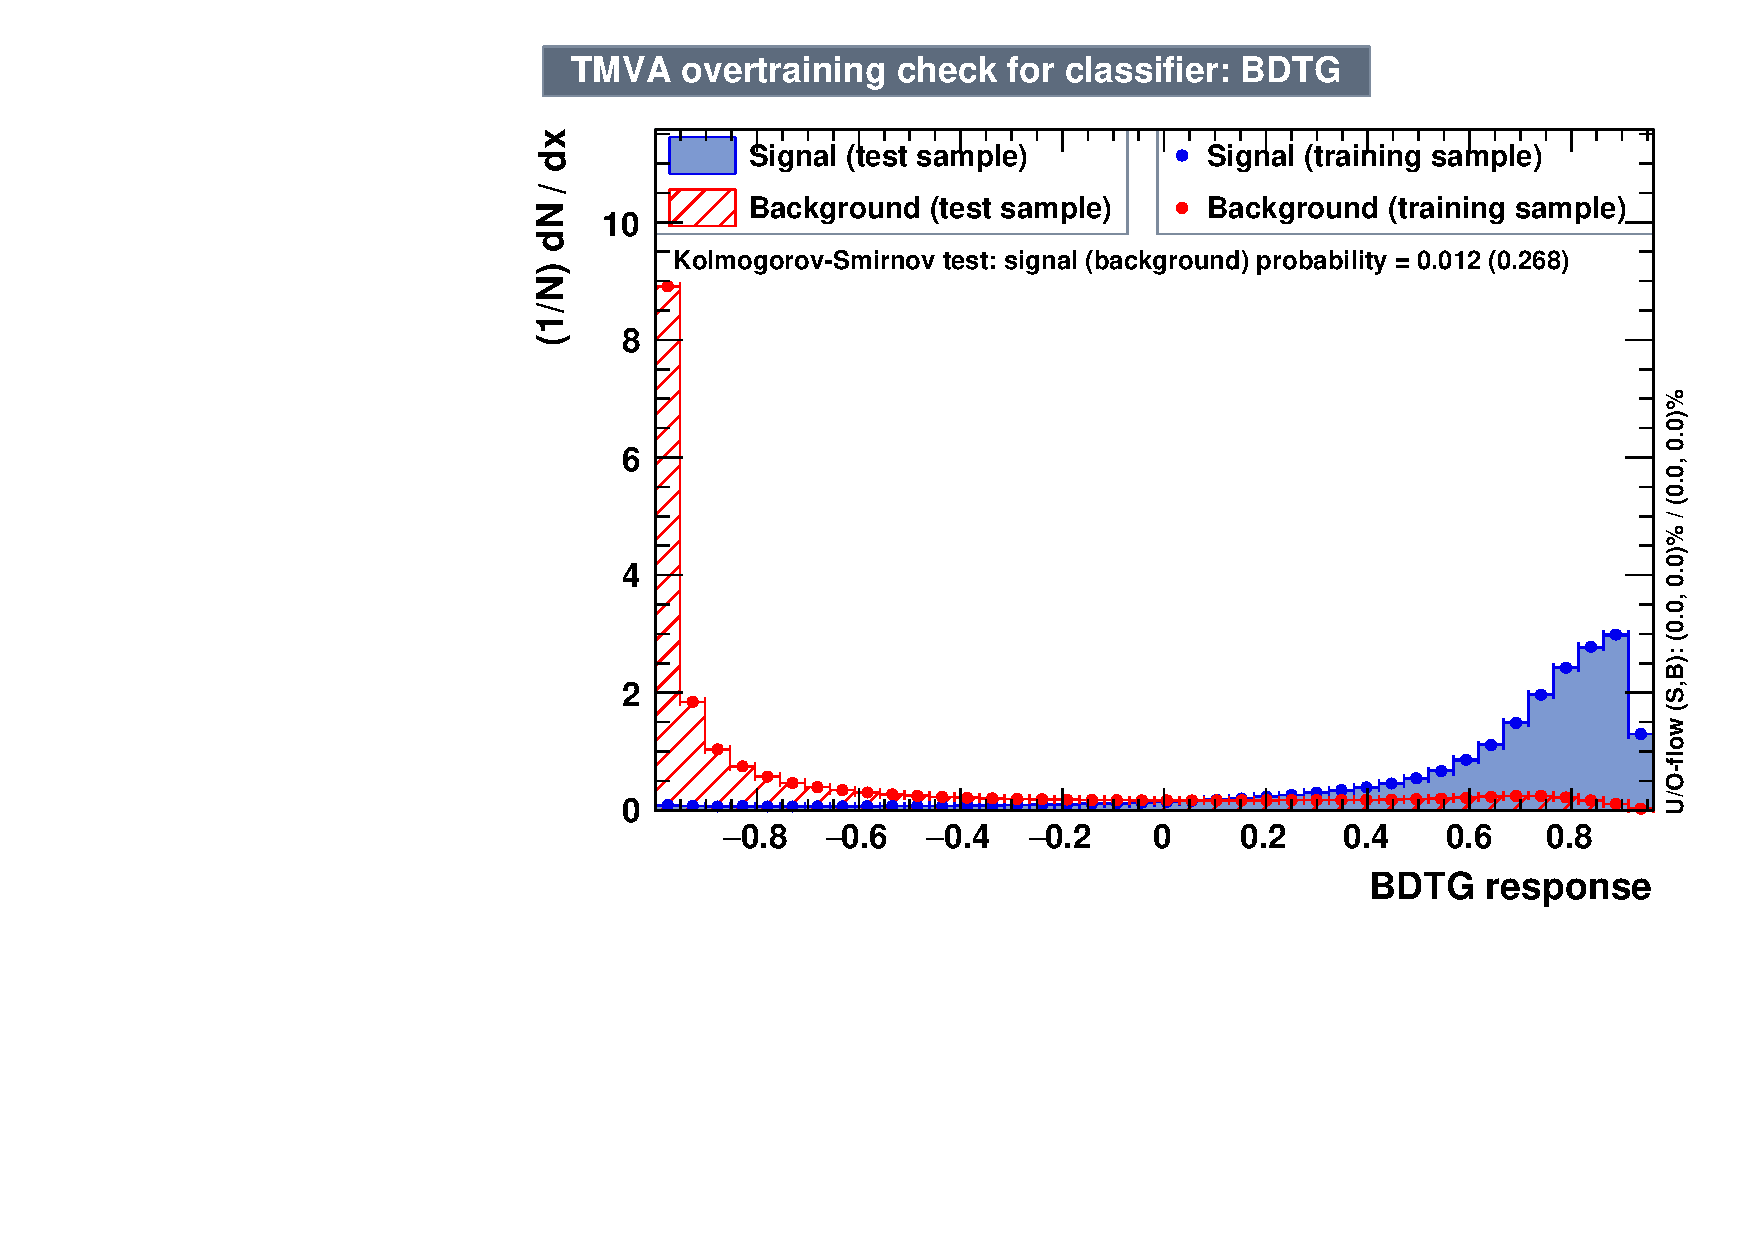
\includegraphics[width=0.45\textwidth]{Figures/EventSelReco/a05_all_BDTG_sep.pdf}}\\
			    \subfigure[MLP's separation result]{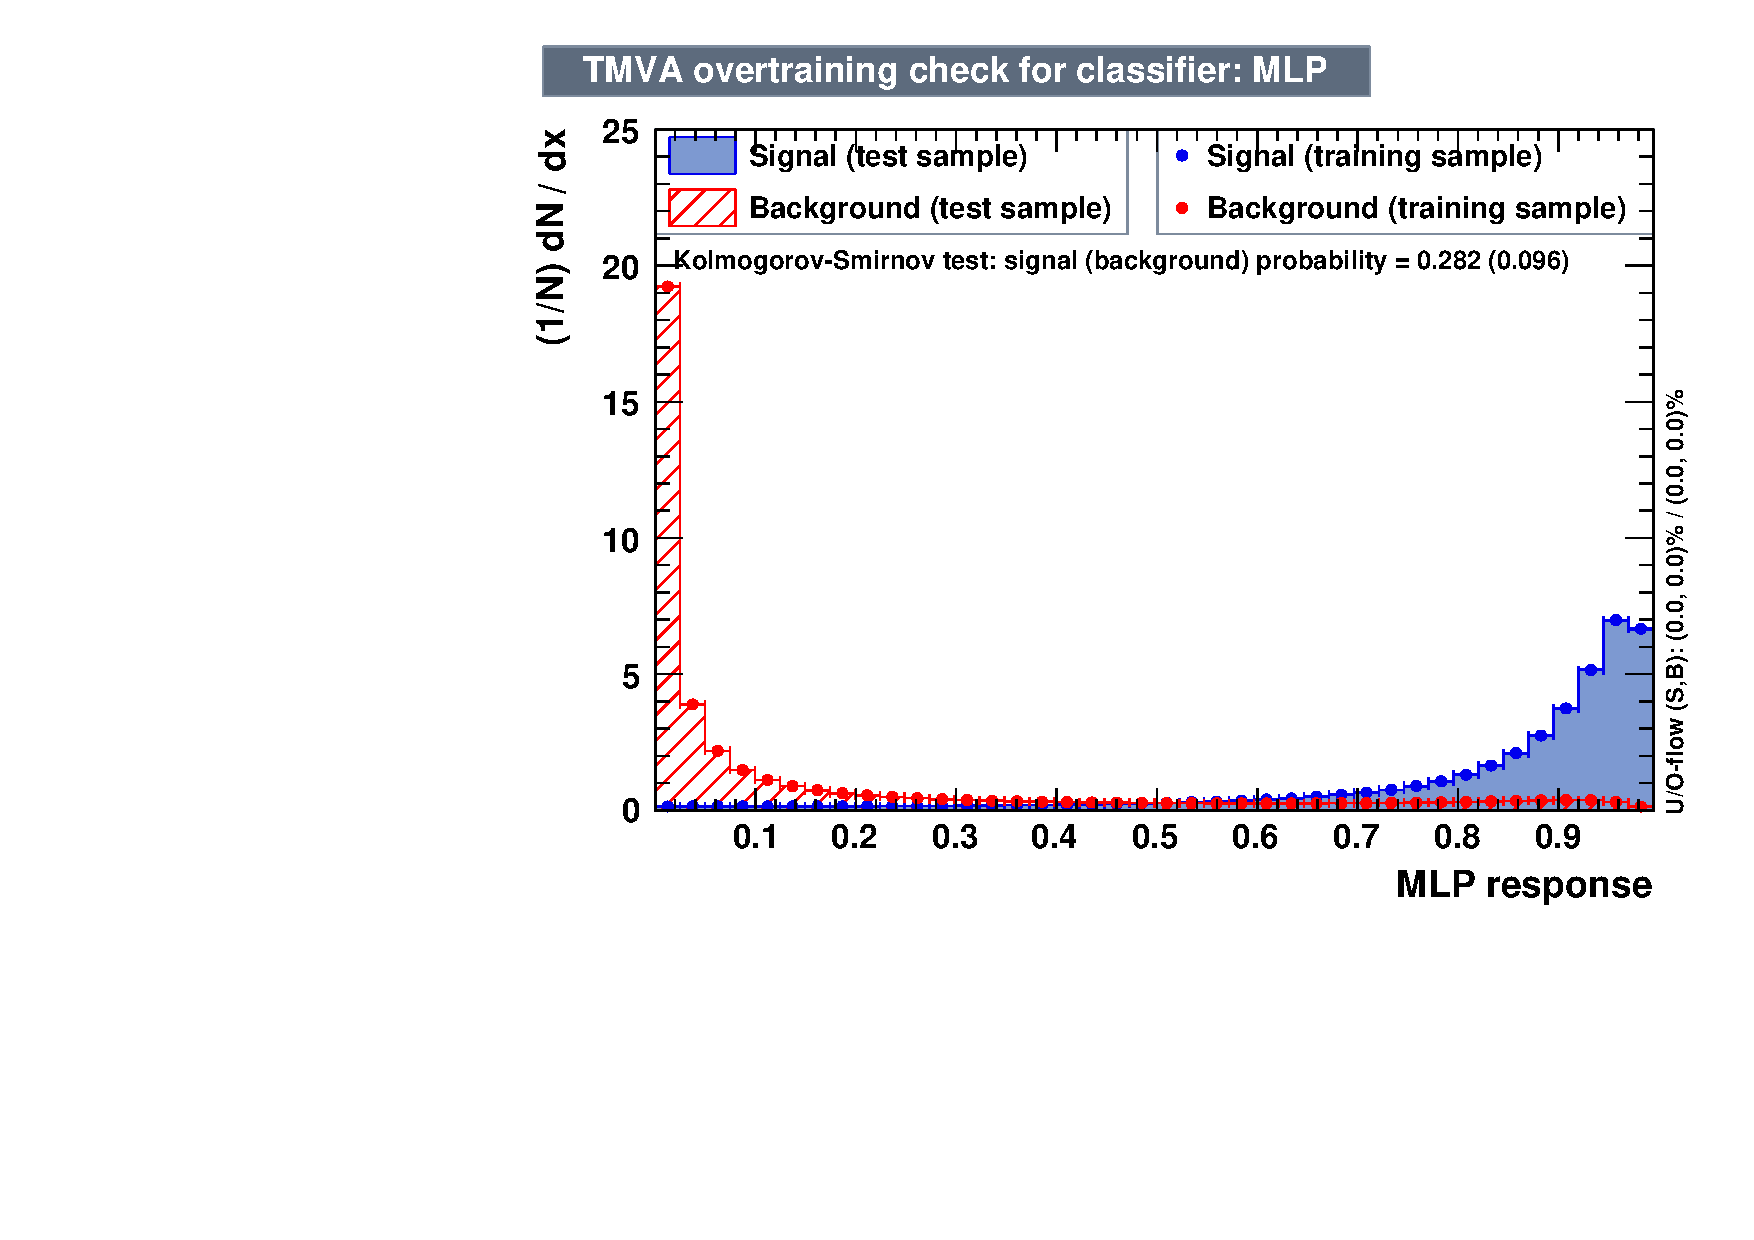
\includegraphics[width=0.45\textwidth]{Figures/EventSelReco/a05_all_MLP_sep.pdf}}
			    \subfigure[ROC curve]{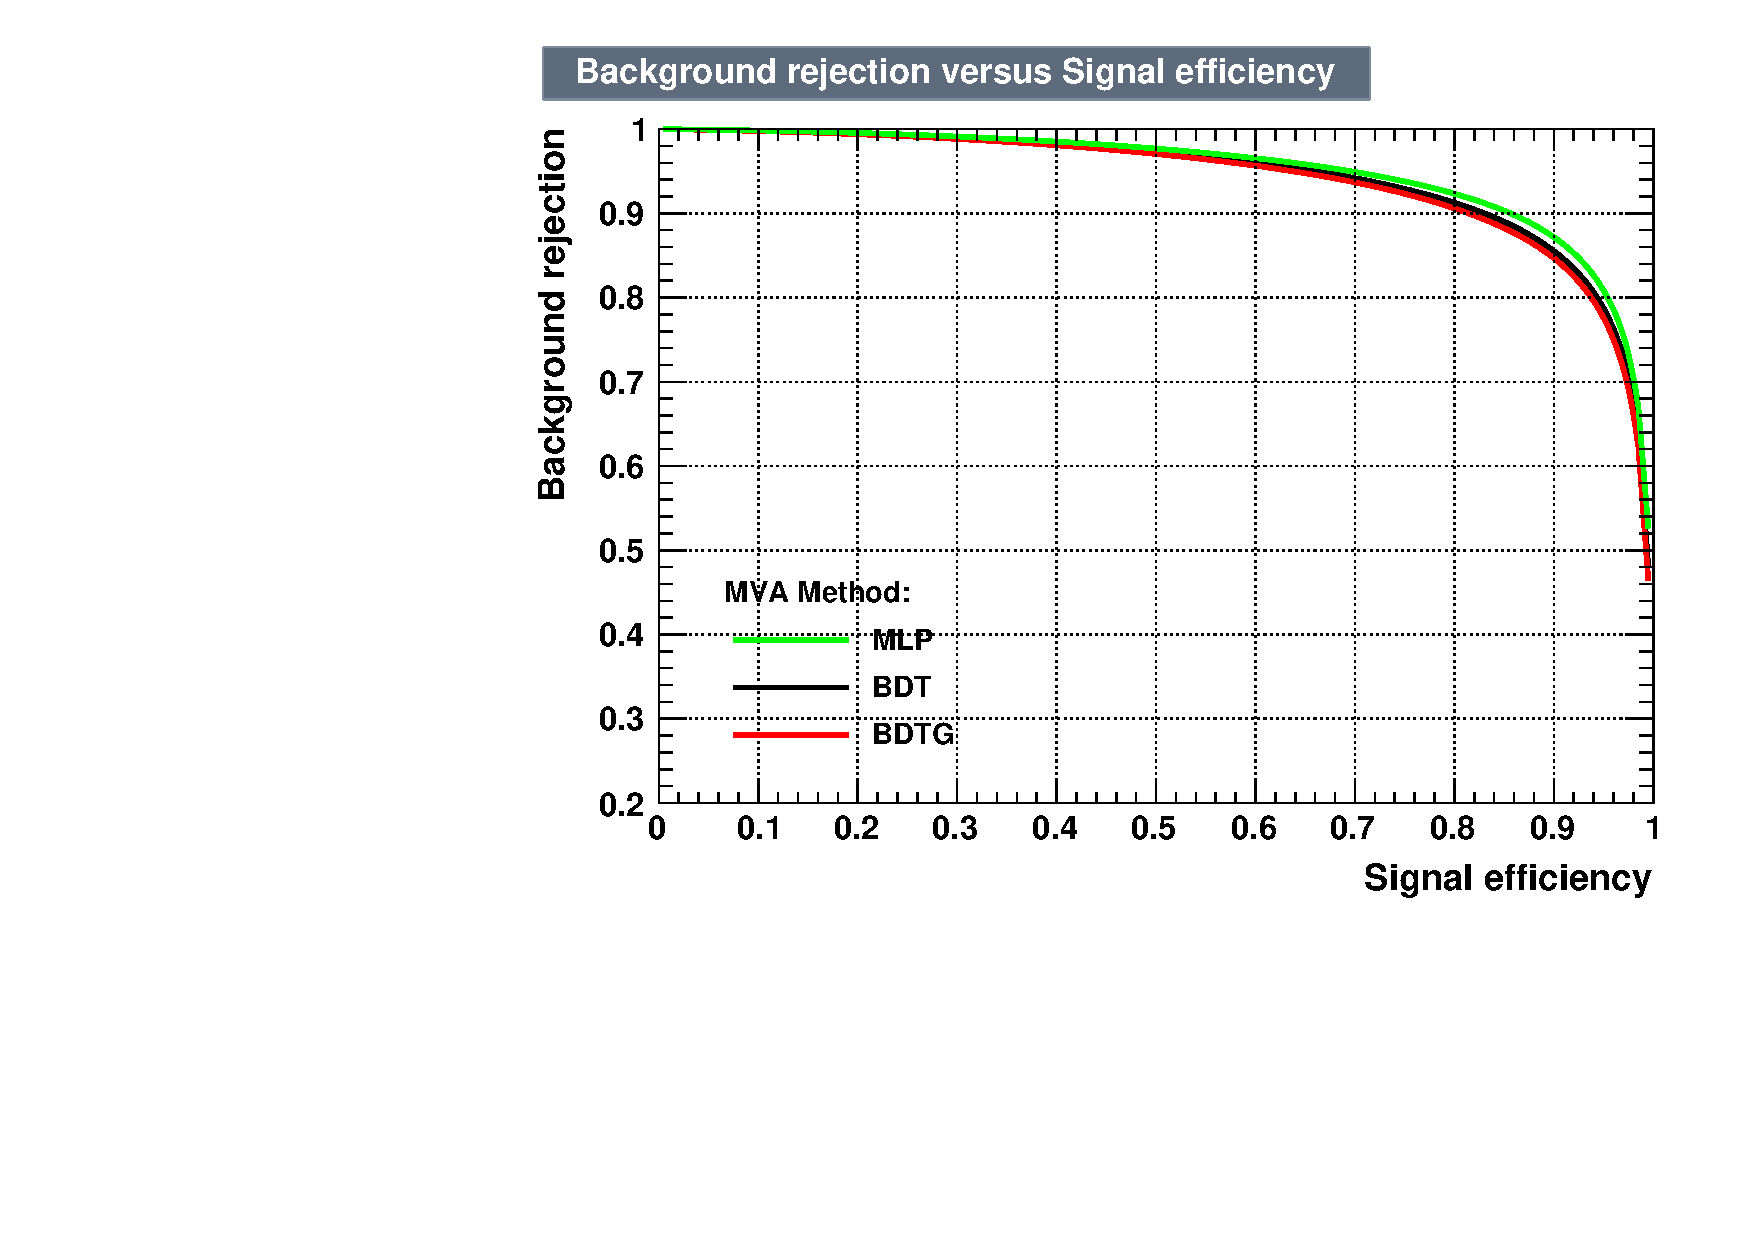
\includegraphics[width=0.45\textwidth]{Figures/EventSelReco/a05_all_ROC.pdf}}\\
			\caption{The training result of 20 variables set}
			\label{EventSelReco:fig:Sep_ROC_a05}
			\end{figure}
			\FloatBarrier

			This is shown that the MLP(ANN) training algorithm has the best performance under ROC criteria from training results. But as previous mentioning, the ROC performance cannot totally represent the training performance completely in these analysis case.

	\subsection{$b\bar{b}$ separation and distinguishment}
	\label{ssec:bbsep}

		The good correctness of chosen physical objects is necessary in this analysis. By the basis for discovering new physics, the observables require precise identification of particles. And the important is, in our selected observables, to distinguish $b$- between $\bar{b}$ -quark which are both b-tagged jets detected from smashing and hadronizatoin of b-flavor quarks. For example, the identification is highly correlated with observable $O_{6}$ which is $q_{l}(\vec{p_{b}}-\vec{p_{\bar{b}}})\cdot(\vec{p_{l}}\times\vec{p_{j_{1}}})$, the mis-ordered $b$/($\bar{b}$) will cause the wrong sign on this observable. On the other hand, it is not requirement for us to correctly pick up the 2 jets from hadronically decaying top quark in this analysis. In this way, the identification between $b$ and $\bar{b}$ is the most critical implication. And that is also what we need to test the performance of reconstruction algorithm($\chi^2_{min}$,MVA). 

		The study is worked under the signal simulation sample($t$$\bar{t}$ Monte Carlo). All the selected physical objects include jets and leptons will be matched to particle with the generator-level information in MC sample with $\Delta R$ < 0.4 method.(Eq.\ref{eq:gen_matching})

		To standardlize the $b$/$\bar{b}$ distinguishment, there are 3 classifications listed:
		\begin{itemize}
  		\item $\textbf{Correct}$: $b$-quark is identified as $b$-jets and $\bar{b}$-quark is identified as $\bar{b}$-jets
  		\item $\textbf{b/}$$\bar{\textbf{b}}$ $\textbf{mis-identified}$: $b$-quark is identified as $\bar{b}$-jets and $\bar{b}$-quark is identified as $b$-jets
  		\item $\textbf{Mistag}$: non $b$$(\bar{b})$-quark is identified as $b$$(\bar{b})$-jet
		\end{itemize}

		With applying the various algorithm on signal simulation sample($t\bar{t}$ MC), there are the $b/\bar{b}$-distinguishment of $\chi^2_{min}$ and MVA methods:

		\begin{center}
		\begin{longtable}[H]{ c c c c c }			% add the [H] can make it listed in table list!!
		\caption{fff}\\
		\hline
		[\%] & & Correct & $b\bar{b}$ mis-identified & Mistag  \\ 
		\hline
		$\chi^2_{min}$ &  & XXX & 1 & CCCCCC \\
		\hline
		\multirow{3}{5em}{2 variables} & MLP & XXX & 2 & CCCCCC \\
		& BDT & XXX & 2 & CCCCCC \\
		& BDTG & XXX & 2 & CCCCCC \\
		\hline
		\multirow{3}{5em}{8 variables} & MLP & XXX & 2 & CCCCCC \\
		& BDT & XXX & 2 & CCCCCC \\
		& BDTG & XXX & 2 & CCCCCC \\
		\hline
		\multirow{3}{5em}{20 variables} & MLP & XXX & 2 & CCCCCC \\
		& BDT & XXX & 2 & CCCCCC \\
		& BDTG & XXX & 2 & CCCCCC \\
		\hline  
		\end{longtable}
		\end{center}



	\subsection{Control Region}
	\label{ssec:CR}


		Those are seen nice after training. Since we will use the spectrum of leptonic top's invariant mass($M_{lb}$) to estimate our signal($t\bar{t}$) and background in Chapter****, it is necessary to retain the isolation of information about $M_{lb}$ when reconstructing the hadronic top mass $M_{jjb}$. There is a check to see if a cut on mva score is given, whether the $M_{lb}$'s pdf(probability density function) shape change. If the cut on mva score which is designed and trained for reconstructing $M_{jjb}$ would vary the $M_{lb}$ shape, there are some obvious interference from reconstructing $M_{jjb}$ to information of $M_{lb}$. That is what we need to circumvent for following analysis strategy.

		\begin{figure}[H]
		\end{figure}
		\FloatBarrier


\FloatBarrier
